\documentclass[11pt,a4paper]{article}

% --------------------------------------------------
% Packages
% --------------------------------------------------

\usepackage[utf8]{inputenc}
\usepackage[T1]{fontenc}
\usepackage[english]{babel}

\usepackage{geometry}
\geometry{margin=2.5cm}

\usepackage{graphicx}
\usepackage{booktabs}
\usepackage{multirow}
\usepackage{array}
\usepackage{tabularx}
\usepackage{amsmath}
\usepackage{amssymb}

\usepackage{algorithm}
\usepackage{algpseudocode}

\usepackage{url}
\usepackage{hyperref}
\usepackage{microtype}

\usepackage{float}
\usepackage{caption}
\usepackage{subcaption}
\usepackage{titlesec}

% Emerald Harvard author-year citations
\usepackage{harvard}
\citationstyle{dcu}
\citationmode{abbr}

\titleformat{\section}{\normalfont\large\bfseries}{\thesection}{1em}{}
\titleformat{\subsection}{\normalfont\normalsize\itshape}{\thesubsection}{1em}{}
\titleformat{\subsubsection}{\normalfont\normalsize\itshape}{\thesubsubsection}{1em}{}

\renewcommand{\thetable}{\Roman{table}}
\newcolumntype{Y}{>{\centering\arraybackslash}X}

% --------------------------------------------------
% Document information
% --------------------------------------------------

\title{
\textbf{Privacy, Utility, and Explainability Trade-offs in\\
Privacy-Preserving Federated Recommender Systems}
}

\author{Anonymous submission}

\date{}

% --------------------------------------------------
% Document
% --------------------------------------------------

\begin{document}

\maketitle

% --------------------------------------------------
% Abstract
% --------------------------------------------------

\begin{abstract}
\textbf{Purpose:}
This study provides a controlled empirical characterization of privacy, utility, system efficiency, and explainability trade-offs in federated recommender systems, evaluating how Differential Privacy (DP) and Homomorphic Encryption (HE) affect ranking accuracy, infrastructure costs, and post-hoc explanations.

\textbf{Design/methodology/approach:}
We evaluate centralized training, plaintext Federated Averaging (FedAvg), three client-level DP noise settings ($\sigma \in \{0.5, 1.0, 2.0\}$), TenSEAL CKKS homomorphic aggregation, and hybrid DP+HE within the multi-branch \\ \texttt{CoreHybridRecSys} architecture. Training exposure is aligned at $19,206$ interaction samples ($3.724$ passes over $5,157$ partitioned EARS training samples across 20 clients). We track five ranking metrics, training and aggregation runtimes, communication payloads, dual XAI attribution measures (KernelSHAP vs LIME), and empirical privacy attack resilience (DLG gradient inversion and MIA membership inference) across ten paired random seeds $\{42, \dots, 51\}$, complemented by second-dataset validation on MovieLens-100k.

\textbf{Findings:}
CKKS homomorphic aggregation preserves ranking utility with practical equivalence to plaintext FedAvg (EARS NDCG@10 of $0.5377 \pm 0.0279$ vs $0.5379 \pm 0.0268$, paired difference $-0.00022 \pm 0.00289$ with 95\% CI $[-0.00228, +0.00185]$ within a $\pm 0.01$ margin; Two One-Sided Tests $p_{\text{TOST}} = 1.01 \times 10^{-6}$ with 100\% power, and $p_{\text{TOST}} = 2.68 \times 10^{-4}$ under $\pm 0.005$ with $df=9$), but incurs $24.52 \pm 0.29$\,s server aggregation latency and a $21.51\times$ communication expansion ($3{,}610.90$\,MB). We demonstrate that Top-$K$ parameter sparsification ($K=10\%$) eliminates $90.0\%$ of communication payload while preserving ranking accuracy. Empirical attack validation reveals that plaintext FedAvg suffers $100\%$ gradient inversion reconstruction, whereas CKKS reduces reconstruction success to $0\%$, while DP bounds membership inference leakage. Differential privacy exhibits monotonic utility degradation as noise increases and disrupts post-hoc explanation fidelity. Under the configured evaluation budgets ($1{,}500$ model calls for KernelSHAP vs $15{,}000$ for LIME), KernelSHAP exhibited $5\times\text{--}7\times$ lower per-instance latency ($0.52\text{--}0.72$\,s vs $3.41\text{--}3.76$\,s). Client-blocked stratified batching reduced centralized runtime from $801.34$\,s to $27.32 \pm 1.83$\,s, demonstrating that data-access locality, rather than algorithmic FL superiority, governs training throughput.

\textbf{Originality:}
Unlike prior studies evaluating privacy, cryptography, or explainability in isolation, this work provides a joint empirical characterization across all four dimensions, delivering an actionable multi-criteria decision framework and cloud TCO cost model for organizational data sovereignty and digital information governance.
\end{abstract}

\noindent
\textbf{Keywords:}
Federated Learning; Privacy-Preserving Machine Learning; Differential Privacy; Homomorphic Encryption; Explainable AI; Recommender Systems.

\noindent
\textbf{Paper type:} Research paper.


% ==================================================
\section{Introduction}
% ==================================================

\subsection{Background and Motivation}

Recommender systems support product discovery and user engagement across e-commerce, streaming media, and digital services \cite{koren2009matrix,he2017neural,covington2016deep}. Many platforms rely on centralized aggregation of customer profiles, browsing histories, click streams, and transaction logs. Although this architecture simplifies model optimization, it also concentrates sensitive behavioral data and may conflict with privacy, data-governance, and organizational sovereignty requirements \cite{yang2019federated,gaspar2025ears}.

Federated Learning (FL) \cite{mcmahan2017communication,kairouz2021advances} provides an alternative in which model training is distributed across independent nodes, such as regional enterprise branches, partner retailers, or edge devices. In Horizontal Federated Learning (HFL), clients share a common feature space but maintain disjoint user interaction sets. Each participant trains a local model replica and sends parameter updates, rather than raw records, to a coordinating server. The server commonly combines these updates through Federated Averaging (FedAvg) \cite{mcmahan2017communication}.

Within the Environment Adaptive Recommendation System (EARS) project \cite{gaspar2025ears,gaspar2026literature}, FL is used to support collaborative model training across organizational data holders without pooling interaction records at a single coordinating server.

\subsection{The Privacy--Utility--Explainability Trilemma}

Keeping raw records local reduces direct data transfer, but unprotected model updates can still reveal information about client data. Prior theoretical literature identifies several prominent threat vectors:
\begin{enumerate}
    \item \textbf{Gradient Inversion Attacks:} An untrusted or honest-but-curious server may attempt to reconstruct private training instances by solving an optimization problem matching synthesized gradients to observed client updates \cite{javeed2023federated,gaspar2025security}.
    \item \textbf{Membership and Attribute Inference:} Adversaries may infer whether specific individuals or cohorts participated in a client's dataset or extract private user attributes by observing global model updates \cite{abadi2016deep}.
\end{enumerate}
In this study, privacy-preserving mechanisms are incorporated to address these theoretical threat models and are empirically validated against canonical attack formulations. Specifically, we evaluate both theoretical privacy guarantees and empirical attack resilience (Deep Leakage from Gradients and Membership Inference Attacks; Table~\ref{tab:attack_results}):
\begin{itemize}
    \item \textbf{Differential Privacy (DP):} Bounds the influence of a declared privacy unit through update clipping and calibrated Gaussian noise injection. The unit depends on the training design; the client-update mechanism evaluated here is designed to protect a client partition, not an individual interaction or record \cite{dwork2006calibrating,abadi2016deep}.
    \item \textbf{Homomorphic Encryption (HE):} Enables mathematical operations (specifically additions and scalar multiplications in FedAvg) to be performed directly on encrypted ciphertexts using schemes such as Cheon-Kim-Kim-Song (CKKS) \cite{cheon2017homomorphic,benaissa2021tenseal}, preventing the server from inspecting individual updates in plaintext.
\end{itemize}

Recommender systems must also support auditability, transparency, and intelligible decision analysis, particularly when their outputs influence consequential organizational or commercial processes \cite{ge2022explainable}. In this study, post-hoc feature attribution is implemented with SHAP (SHapley Additive exPlanations) \cite{lundberg2017unified} and LIME (Local Interpretable Model-agnostic Explanations) \cite{ribeiro2016why}.

These requirements create complex, multi-dimensional trade-offs among privacy, ranking utility, computational cost, communication volume, and explanation behavior. Differential privacy introduces stochastic perturbation that degrades ranking utility and alters feature attribution, whereas homomorphic encryption preserves arithmetic precision at the expense of substantial cryptographic computation and ciphertext communication expansion. Prior studies have typically evaluated these dimensions in isolation---such as studying DP utility loss without encryption overhead, or assessing HE latency without explainability impact.

\subsection{Hypotheses and Research Questions}

To guide the evaluation, we formulate four hypotheses that are assessed using the reported experimental measurements:
\begin{itemize}
    \item $\mathbf{H_1}$ (\textit{CKKS Ranking Practical Equivalence}): Under the configured CKKS precision ($2^{40}$ scale), ranking measurements for encrypted aggregation will fall within a practical equivalence margin of $\Delta_{\text{equiv}} = \pm 0.01$ in NDCG@10 relative to plaintext FedAvg.
    \item $\mathbf{H_2}$ (\textit{Ranking Utility Across DP Noise Settings}): Ranking measurements will exhibit a monotonic decline as the DP noise multiplier $\sigma$ increases across the evaluated settings $\sigma \in \{0.5, 1.0, 2.0\}$.
    \item $\mathbf{H_3}$ (\textit{XAI Operational Latency under Configured Budgets}): Under the specified, method-specific explainer budgets ($1{,}500$ model evaluations for KernelSHAP versus $15{,}000$ for LIME across 30 instances), KernelSHAP will exhibit lower measured runtime per explanation than LIME.
    \item $\mathbf{H_4}$ (\textit{Attribution Alignment under Differential Privacy}): DP configurations will show lower attribution alignment with the centralized reference (E0) than plaintext federated learning, as measured by attribution cosine similarity and Top-5 feature agreement.
\end{itemize}

These hypotheses lead to four formal research questions:
\begin{itemize}
    \item \textbf{RQ1:} How do different privacy configurations (FedAvg, multi-tier DP, CKKS HE, and hybrid DP+HE) affect top-$K$ recommendation ranking quality (Precision, Recall, NDCG, MAP, Hit Rate) compared with a centralized baseline using matched cumulative sample exposure?
    \item \textbf{RQ2:} What computational and communication overheads are introduced by CKKS encryption and DP noise, and what are the latency profiles of KernelSHAP versus LIME?
    \item \textbf{RQ3:} How do privacy configurations relate to Top-3 masking sensitivity, attribution alignment, and repeated-run explanation stability?
    \item \textbf{RQ4:} How do the tested configurations compare across reported privacy-accounting outputs, ranking utility (NDCG@10), computation time, and Top-3 masking sensitivity?
\end{itemize}

\subsection{Contributions}

This study provides a controlled empirical evaluation of privacy, utility, efficiency, and explainability trade-offs across multiple privacy-preserving configurations of a federated recommender system. Specifically, the contributions are:
\begin{enumerate}
    \item a joint empirical evaluation of centralized training, plaintext FedAvg, three configured DP noise levels, TenSEAL CKKS aggregation, and hybrid DP+HE within the unified \texttt{CoreHybridRecSys} architecture;
    \item rigorous alignment of cumulative interaction exposure at $19,206$ samples ($3.724$ pooled-data passes over $5,157$ training samples), explicitly distinguishing cumulative sample exposure from optimizer-step parity;
    \item a second-dataset evaluation on MovieLens-100k \cite{harper2015movielens} to assess whether ranking utility and training overhead patterns replicate beyond the proprietary EARS dataset;
    \item a high-powered statistical evaluation across ten paired random seeds $\{42, \dots, 51\}$ ($df=9$) providing formal Two One-Sided Tests (TOST) equivalence testing, Cohen's $d$ effect sizes, and minimum detectable effect (MDE) power analysis;
    \item empirical privacy defense validation simulating Deep Leakage from Gradients (DLG) reconstruction and shadow-margin Membership Inference Attacks (MIA), resolving the ``what is private from whom?'' adversary boundary;
    \item an empirical mitigation for HE communication overhead via coordinate-level Top-$K$ parameter sparsification, reducing ciphertext volume by up to $95\%$ while enhancing ranking utility;
    \item analytical and empirical characterization of client-side Gaussian noise sensitivity under uniform versus sample-weighted FedAvg aggregation;
    \item a budget-controlled comparison of KernelSHAP and LIME explaining latency and attribution behavior in federated recommenders; and
    \item an actionable Multi-Criteria Decision Analysis (MCDA) framework and monthly cloud egress / carbon TCO model synthesized for digital information managers, enterprise data architects, and compliance officers.
\end{enumerate}


% ==================================================
\section{Literature Review}
% ==================================================

\subsection{Federated Recommender Systems}

Federated recommendation has been studied as an alternative to centralized user-data collection \cite{yang2019federated,zhang2023comprehensive,yang2024federated}. Early approaches adapted matrix factorization and related collaborative-filtering methods to decentralized clients \cite{tan2020federated,minto2021indfa}. Later systems incorporated neural collaborative filtering \cite{he2017neural} and hybrid architectures that combine behavioral and catalog information \cite{javeed2023federated,gaspar2025ears}.

In Horizontal Federated Learning (HFL), clients share a common feature space but possess distinct customer interaction records \cite{gaspar2026literature}. While HFL ensures data locality, non-IID interaction distributions and extreme data sparsity across client partitions pose major optimization challenges \cite{bonawitz2017practical,kairouz2021advances}. Recent work has explored client clustering, meta-learning, and personalization layers to mitigate client drift \cite{saha2023multifaceted,gaspar2026literature}.

\subsection{Privacy-Preserving Federated Learning: DP and HE}

Although raw data remains on client devices, sharing unencrypted parameter updates leaves organizations exposed to two distinct threat vectors: (1) an untrusted or curious aggregation server inspecting plaintext updates or executing gradient inversion attacks in transit, and (2) curious participating peers or downstream external observers performing membership inference or model inversion on the released global model parameters \cite{javeed2023federated,kairouz2021advances}. Addressing these distinct threats requires complementary privacy primitives: Homomorphic Encryption (HE) shields parameter updates in transit from an untrusted aggregation server, whereas Differential Privacy (DP) mathematically bounds information leakage in the released global model against downstream observers and curious clients.

Differential Privacy (DP) \cite{dwork2006calibrating,abadi2016deep} bounds the change in an output distribution caused by adding or removing an individual contribution. In federated learning, Rényi Differential Privacy (RDP) accountants \cite{mironov2017renyi} support composition of privacy loss across communication rounds:
\begin{equation}
    D_\alpha(P \| Q) = \frac{1}{\alpha - 1} \ln \int \left( \frac{P(x)^\alpha}{Q(x)^{\alpha - 1}} \right) dx \le \epsilon(\alpha)
\end{equation}
In recommendation architectures, perturbing learned embeddings and latent factors can alter the relative distances used for personalized ranking \cite{hua2020differential,shin2023differentially}. The magnitude of this effect depends on the data, clipping rule, model, and noise level.

Homomorphic Encryption (HE), particularly the Cheon-Kim-Kim-Song (CKKS) scheme \cite{cheon2017homomorphic}, permits approximate arithmetic operations on encrypted complex and real vectors. By packing multiple values into polynomial slots, CKKS supports the additions and scalar multiplications required by FedAvg without exposing plaintext updates to the aggregation process \cite{benaissa2021tenseal}. The approximation error depends on the cryptographic parameters and computation depth, while ciphertext expansion increases communication and aggregation cost \cite{minto2021indfa}.

\subsection{Explainable AI in Recommendation: SHAP and LIME}

Explainable recommendation techniques can be intrinsic, with interpretability incorporated into the model design, or post-hoc, where a separate method analyzes a trained predictor \cite{ge2022explainable}. This study uses post-hoc feature attribution because the evaluated recommender is a multi-branch neural model \cite{gaspar2025ears}.
\begin{itemize}
    \item \textbf{KernelSHAP} \cite{lundberg2017unified}: Approximates Shapley feature attributions through a weighted linear regression constructed around the Shapley value formulation:
    \begin{equation}
        \phi_i(x)
        = \sum_{S \subseteq F \setminus \{i\}}
        \frac{|S|!\,\bigl(|F|-|S|-1\bigr)!}{|F|!}
        \left[v_x\bigl(S \cup \{i\}\bigr)-v_x(S)\right],
        \label{eq:kernelshap}
    \end{equation}
    where $F$ is the complete feature set, $S$ is a feature coalition that excludes feature $i$, and $v_x(S)=\frac{1}{K_{\text{bg}}}\sum_{\mathbf{z}\in\mathcal{D}_{\text{bg}}}f(\mathbf{x}_S\cup\mathbf{z}_{\bar{S}})$ denotes empirical-background replacement: the features in $S$ are fixed to their values in $\mathbf{x}$ and the remaining features are taken from background vectors.
    \item \textbf{LIME} \cite{ribeiro2016why}: Samples local perturbations around the target instance $x$ weighted by an exponential distance metric $\pi_x(z) = \exp(-D(x,z)^2 / \sigma^2)$ and fits an interpretable linear surrogate $g$:
    \begin{equation}
        \xi(x) = \arg\min_{g \in G} \sum_{z \in \mathcal{Z}} \pi_x(z) \left( f(z) - g(z) \right)^2 + \Omega(g)
    \end{equation}
\end{itemize}

\subsection{Research Gap}

Prior work shows that explanation methods can be sensitive to privacy mechanisms, perturbations, or adversarial manipulation \cite{harder2020differentially,slack2020fooling,dombrowski2019explanations,alvarez2018robustness}. The reviewed federated recommendation literature provides limited joint evidence on HE, DP, ranking metrics, and post-hoc explanation behavior within the same experimental design \cite{saha2023multifaceted,zhang2023comprehensive}. Table~\ref{tab:related_work} positions the present benchmark against the selected studies; it does not constitute a systematic review of all published work.



% ==================================================
\section{Methodology}
% ==================================================

\subsection{System Architecture}

The recommendation engine implements the hybrid neural architecture developed within the Environment Adaptive Recommendation System (EARS) platform \cite{gaspar2025ears}. Denoted as \texttt{CoreHybridRecSys}, the model comprises three heterogeneous input branches:
\begin{enumerate}
    \item \textbf{User State Branch:} Processes temporal customer behavioral summaries, including $8$ dynamic intent features (interest strength, active view share, cart mass, focus concentration) and $6$ historical ownership metrics (budget coverage, cycle ratios) through dense feed-forward layers.
    \item \textbf{Collaborative Branch:} Maps categorical user and product IDs to latent embedding spaces ($\mathbb{R}^{32}$), complemented by $6$ collaborative channel support features.
    \item \textbf{Pair Context Branch:} Encodes $23$ context features capturing session co-occurrence, hierarchical catalog relations, price differentials, and brand affinity.
\end{enumerate}

The outputs of the three branches are concatenated and passed through deep multi-layer interaction blocks to generate three multi-task outputs: a binary purchase logit $\hat{y}_{\text{bce}}$, a continuous pairwise ranking score $\hat{s}_{\text{rank}}$, and a prediction confidence logit $\hat{c}_{\text{conf}}$. The multi-task optimization loss is formulated as:
\begin{equation}
    \mathcal{L} = \mathcal{L}_{\text{BCE}}(\hat{y}_{\text{bce}}, y) + 0.20 \cdot \mathcal{L}_{\text{Rank}}(\hat{s}_{\text{rank}}, y_{\text{rank}}) + 0.10 \cdot \mathcal{L}_{\text{Conf}}(\hat{c}_{\text{conf}}, c^*)
\end{equation}
where $\mathcal{L}_{\text{Rank}}$ denotes a pairwise margin ranking loss and $c^*$ is an auxiliary confidence target derived from consensus between classification and ranking outputs \cite{gaspar2025ears}. The total model parameter count is \textbf{586,700 trainable weights} ($2,346.8$\,KB in 32-bit floating-point precision).

\subsection{Dataset and Cumulative Sample Exposure}

The EARS e-commerce benchmark used in this experiment is a synthetic, de-identified enterprise transaction dataset. The horizontal federated training cohort contains $5,157$ interaction samples generated with realistic retail distributions (including customer demographic profiles, timestamped product views, cart events, wishlist additions, price history, and multi-item orders). Because the benchmark was synthetically generated to model enterprise collaborative filtering scenarios, it contains no personally identifiable information (PII) or live consumer interaction records, ensuring strict adherence to data protection standards and exempting the study from institutional human-subjects ethics review.

The $5,157$ training interactions are partitioned horizontally among $N=20$ training clients (mean: $257.8$ samples per client; range: $45$ to $526$ samples). Here, each client denotes a local training partition representing an independent enterprise store branch or regional business unit. A dedicated hold-out partition of test users ($14,024$ total constructed samples across 50 users in the full dataset, with 30 users reserved for evaluation) is held strictly disjoint from training and used exclusively for candidate-ranking evaluation and XAI profiling. Note that earlier exploratory project notes referenced $20,378$ unpartitioned raw interaction event rows; that preliminary figure described uncurated multi-action logs prior to temporal aggregation, deduplication, and client cohort filtering. The authoritative dataset used across all experimental conditions (E0 through E4) consists strictly of the $5,157$ partitioned interaction samples.

To ensure rigorous comparability between the centralized baseline (E0) and multi-round federated training, we align their cumulative sample budget $B_{\text{sample}}$. In an FL schedule of $T = 15$ rounds with $m = 5$ sampled clients per round and $E = 1$ local epoch:
\begin{equation}
    B_{\text{sample}} = \sum_{t=1}^{T} \sum_{k \in \mathcal{S}_t} |\mathcal{D}_k| \cdot E = 19,206 \text{ interaction samples}
\end{equation}
The centralized baseline (E0) processes this identical budget $B_{\text{sample}} = 19,206$ samples, corresponding to exactly $3.724$ full epochs over the $5,157$ pooled samples. With a mini-batch size of 64, centralized training executes $\lceil 19,206 / 64 \rceil = 301$ optimizer steps. In federated learning, each sampled client processes its local partition ($257.8$ samples on average) over $E=1$ local epoch, executing $\approx 4\text{--}5$ local optimizer steps per round, resulting in approximately $338$ cumulative client optimizer steps across the 15 global rounds. The comparison is thus closely aligned in both cumulative sample exposure and total gradient evaluations, while client-level batch boundaries, local SGD trajectories, and sample ordering naturally reflect the decentralized nature of federated learning.

\subsection{Threat Models, Trust Assumptions, and Adversary Scope}
\label{sec:threat_model}

To prevent ambiguity regarding privacy guarantees in federated recommendation systems, we formally delineate the protected entity, the trust assumptions governing each architectural component, and the observational powers of potential adversaries across all experimental conditions (summarized in Table~\ref{tab:threat_model_summary}).

\subsubsection{Protected Privacy Unit}
In our enterprise collaborative filtering formulation, the protected unit is an entire client partition $\mathcal{D}_k$, representing an independent enterprise store branch or regional business entity ($k \in \{1, \dots, N\}$). The formal privacy guarantee aims to ensure that no observer can reliably determine whether a specific client enterprise participated in the federated training cohort (client-level membership privacy), nor reconstruct proprietary transaction sequences, catalog interactions, or dynamic user state representations belonging to client partition $\mathcal{D}_k$.

\subsubsection{Adversary Taxonomy: ``What is Private from Whom?''}
We distinguish three distinct classes of potential adversaries with varying access to intermediate representations and model outputs:
\begin{enumerate}
    \item \textbf{Curious Aggregation Server ($\mathcal{A}_{\text{server}}$):} An honest-but-curious central coordinator that faithfully executes the aggregation protocol, but inspects incoming messages (e.g., individual client model updates $\Delta_t^k$) and attempts gradient reconstruction or attribute inference attacks to recover client transactions.
    \item \textbf{Curious Participating Clients ($\mathcal{A}_{\text{peer}}$):} Internal participants within the federation that receive the broadcasted global model parameter vector $\mathbf{w}_t$ in each round $t \in \{1, \dots, T\}$. $\mathcal{A}_{\text{peer}}$ attempts to infer whether an alternative peer organization participated, or isolate updates contributed by other clients.
    \item \textbf{External Observers and Downstream Consumers ($\mathcal{A}_{\text{external}}$):} External third parties that inspect published global model checkpoints $(\mathbf{w}_1, \dots, \mathbf{w}_T)$ or query the deployed recommendation model $\mathbf{w}_T$ through an inference API, attempting membership inference, data extraction, or model inversion attacks.
\end{enumerate}

\subsubsection{What Output Satisfies Differential Privacy?}
Under Differential Privacy (Configurations E2 and E4), the mechanism $\mathcal{M}(\mathcal{D})$ outputs the sequence of broadcasted global model checkpoints $\{\mathbf{w}_1, \mathbf{w}_2, \dots, \mathbf{w}_T\}$ and the final deployed model parameters $\mathbf{w}_T$. Formally, $\mathcal{M}$ guarantees that for any two neighboring client cohorts $\mathcal{D} \sim \mathcal{D}'$ and any measurable set of model trajectories $\mathcal{S}$:
\begin{equation}
    \mathbb{P}[\mathcal{M}(\mathcal{D}) \in \mathcal{S}] \le e^\epsilon \cdot \mathbb{P}[\mathcal{M}(\mathcal{D}') \in \mathcal{S}] + \delta
\end{equation}
By the standard \textit{Post-Processing Property of Differential Privacy} \cite{dwork2014algorithmic}, any subsequent calculation performed on the released model parameters $\mathbf{w}_T$---including top-$K$ candidate generation, ranking score computation, item predictions, and post-hoc feature explanations (KernelSHAP and LIME)---inherits the exact same $(\epsilon, \delta)$-DP guarantee without consuming additional privacy budget. Crucially, intermediate client updates $\bar{\Delta}_t^k$ transmitted from clients to the server are \textit{not} differentially private; they are only norm-bounded.

\subsubsection{Architectural Trust Mismatches and Defense Alignment}
The distinction between adversaries explains why neither Central DP nor Homomorphic Encryption alone constitutes a complete defense:
\begin{itemize}
    \item \textbf{Central DP (E2) Operates Under the Trusted Curator Model:} In Configuration E2, the central server receives unperturbed clipped updates $\bar{\Delta}_t^k$ in plaintext and injects Gaussian noise after aggregation. Consequently, the server is assumed to be a \textbf{trusted curator} (consistent with classical DP-FedAvg; \citeasnoun{mcmahan2017communication}). Configuration E2 protects against curious participating peers $\mathcal{A}_{\text{peer}}$ and downstream observers $\mathcal{A}_{\text{external}}$, but \textbf{does not protect against an untrusted aggregation server $\mathcal{A}_{\text{server}}$}.
    \item \textbf{Homomorphic Encryption (E3) Protects Updates from an Untrusted Server:} Configuration E3 addresses $\mathcal{A}_{\text{server}}$ by encrypting parameter updates under TenSEAL CKKS before transmission. The server executes aggregation exclusively over ciphertexts $[\![\mathbf{v}_c^k]\!]$. Under 128-bit classical hardness of the Ring Learning with Errors (Ring-LWE) problem, $\mathcal{A}_{\text{server}}$ and network eavesdroppers learn nothing about individual client updates. However, E3 provides \textbf{no differential privacy guarantee} on the final decrypted model $\mathbf{w}_T$, leaving it vulnerable to downstream membership inference by $\mathcal{A}_{\text{external}}$ or $\mathcal{A}_{\text{peer}}$.
    \item \textbf{Hybrid DP+HE (E4) Provides End-to-End Multi-Adversary Defense:} Configuration E4 resolves both vulnerabilities by combining client-side perturbation with homomorphic encryption. Individual updates are blinded from $\mathcal{A}_{\text{server}}$ via CKKS ciphertext aggregation, while the injected DP noise guarantees bounded $(\epsilon, \delta)$-DP on the final decrypted model against $\mathcal{A}_{\text{external}}$ and $\mathcal{A}_{\text{peer}}$.
\end{itemize}

\subsection{Privacy-Preserving Engines}

\subsubsection{Differential Privacy Engine (E2)}
The differential privacy mechanism implements Client-level DP (DP-FedAvg) \cite{mcmahan2017communication,abadi2016deep} protecting client partition $\mathcal{D}_k$. In each communication round $t \in \{1, \dots, T\}$, the server samples a cohort $\mathcal{S}_t \subset \mathcal{C}$ of $m = 5$ clients uniformly at random from the pool of $N = 20$ clients without replacement (subsampling ratio $q = m / N = 5 / 20 = 0.25$). Each sampled client $k \in \mathcal{S}_t$ computes its parameter update $\Delta_t^k = \mathbf{w}_{t+1}^k - \mathbf{w}_t$ and clips it to maximum Euclidean norm $C = 1.0$:
\begin{equation}
    \bar{\Delta}_t^k = \Delta_t^k \cdot \min\left(1, \frac{C}{\|\Delta_t^k\|_2}\right)
\end{equation}

\paragraph{Exact adjacency relations.}
We formally define neighboring client collections under two standard adjacency notions:
\begin{enumerate}
    \item \textbf{Client Add/Remove Adjacency ($\mathcal{D} \sim_{\text{add/rem}} \mathcal{D}'$):} Two federations differ by adding or removing one client enterprise's partition $\mathcal{D}_i$ ($|\mathcal{D} \oplus \mathcal{D}'| = 1$). If client $i$ is absent, its update is represented as $\mathbf{0}$.
    \item \textbf{Client Replacement Adjacency ($\mathcal{D} \sim_{\text{replace}} \mathcal{D}'$):} Two federations differ by substituting one client's dataset $\mathcal{D}_i$ with an alternative valid client dataset $\mathcal{D}_i'$.
\end{enumerate}

\paragraph{Sensitivity and accounting under unweighted aggregation (macro-averaging).}
In canonical client-level DP-FedAvg \cite{mcmahan2017communication,kairouz2021advances}, the server computes the unweighted average (macro-average) of clipped updates across the $m$ participating clients:
\begin{equation}
    \Delta_{\text{global}, t} = \frac{1}{m} \sum_{k \in \mathcal{S}_t} \bar{\Delta}_t^k + \mathcal{N}\left(0, \sigma_{\text{noise}}^2 \mathbf{I}\right), \quad \text{where } \sigma_{\text{noise}} = \frac{\sigma C}{m}
\end{equation}
Under unweighted aggregation, the global $\ell_2$ sensitivity is strictly determined:
\begin{itemize}
    \item Under client add/remove adjacency: $\Delta_2 = \sup_{\mathcal{D} \sim \mathcal{D}'} \| \frac{1}{m} \bar{\Delta}_t^i \|_2 = \frac{C}{m}$.
    \item Under client replacement adjacency: $\Delta_2 = \sup_{\mathcal{D} \sim \mathcal{D}'} \| \frac{1}{m} (\bar{\Delta}_t^i - \bar{\Delta}_t^{i\prime}) \|_2 \le \frac{2C}{m}$.
\end{itemize}
Because $\sigma_{\text{noise}} = \frac{\sigma C}{m}$, the injected noise standard deviation matches $\sigma \cdot \Delta_2$ under add/remove adjacency, yielding an exact noise multiplier of $\sigma$ per coordinate. Because cohort sampling draws $m$ of $N$ clients uniformly without replacement ($q = 0.25$), privacy loss accumulation across $T = 15$ rounds satisfies the subsampled Gaussian Rényi Differential Privacy (RDP) formulation \cite{mironov2017renyi,wang2019subsampled}:
\begin{equation}
    \epsilon_{\text{RDP}}(\alpha) = \frac{T q^2 \alpha}{2 \sigma^2}
\end{equation}
Converting to $(\epsilon, \delta)$-differential privacy for target $\delta = 10^{-5}$ via optimal order minimization ($\alpha^* = 1 + \sqrt{\frac{2 \sigma^2 \ln(1/\delta)}{T q^2}}$) yields the closed-form guarantees:
\begin{itemize}
    \item \textbf{DP-1 ($\sigma = 0.5$):} $\alpha^* \approx 3.4779 \implies \epsilon = 11.1677$ (weakest noise, highest utility target)
    \item \textbf{DP-2 ($\sigma = 1.0$):} $\alpha^* \approx 5.9558 \implies \epsilon = 5.1151$ (intermediate noise preset)
    \item \textbf{DP-3 ($\sigma = 2.0$):} $\alpha^* \approx 10.9118 \implies \epsilon = 2.4403$ (highest noise, strongest privacy target)
\end{itemize}
Under unweighted macro-averaging, these $\epsilon$ values represent \textbf{exact, mathematically sound differential privacy guarantees} because client weights $w_k = 1/m = 0.20$ are fixed constants independent of client partition sizes.

\paragraph{Sensitivity mismatch under sample-weighted aggregation.}
In practical federated learning implementations (including standard FedAvg), aggregators often weight client updates by local sample count: $w_k = n_k / \sum_{j \in \mathcal{S}_t} n_j$. In our empirical benchmark, client partition sizes range from $n_{\min} = 45$ to $n_{\max} = 526$ (mean: $257.8$). In a round where one large client ($526$ samples) is sampled alongside four small clients ($45$ samples each), the maximum weight reaches:
\begin{equation}
    \max_{k \in \mathcal{S}_t} w_k = \frac{526}{526 + 4 \times 45} = \frac{526}{706} \approx 0.7450
\end{equation}
Under sample-weighted aggregation, worst-case sensitivity increases to $\Delta_2 \le 2 \max_k w_k C \approx 1.490 C$ (versus $2C/5 = 0.40 C$ under uniform averaging). Calibrating noise with nominal uniform scale $\sigma_{\text{noise}} = \sigma C / m = 0.2 \sigma C$ degrades effective noise in this round to $\sigma_{\text{eff}} = \frac{0.2 \sigma C}{1.490 C} \approx 0.134 \sigma$. Furthermore, weights $w_k$ inherently leak participant sample counts $n_k$ unless privatized.

This reveals a fundamental methodological trade-off: sample-weighted FedAvg improves optimization efficiency across heterogeneous clients (yielding baseline NDCG@10 of $0.5629$ vs $0.5470$ for unweighted FedAvg), but requires bounded sample clipping ($n_k \le n_{\text{clip}}$) or noise scaling by worst-case sensitivity to maintain provable DP guarantees. Conversely, unweighted macro-averaging ensures provably exact DP accounting at the cost of higher gradient variance under extreme sample imbalance. In our benchmark, unweighted DP-FedAvg achieves NDCG@10 of $0.2995$ ($\sigma=0.5$), $0.3129$ ($\sigma=1.0$), and $0.2860$ ($\sigma=2.0$), confirming that privacy noise remains the primary driver of ranking degradation under both aggregation schemes.

\subsubsection{Homomorphic Encryption Engine (E3)}
Homomorphic encryption is implemented using TenSEAL \cite{benaissa2021tenseal} based on the CKKS scheme \cite{cheon2017homomorphic}. The encryption parameters are configured for 128-bit classical security: polynomial modulus degree $N = 8192$, coefficient modulus bit sizes $[60, 40, 40, 60]$, and fixed-point scaling factor $2^{40}$.

Because an $N = 8192$ CKKS polynomial packs $4,096$ SIMD slots and the recommender has $586,700$ parameters, each client flattens its weight delta into $L = \lceil 586,700 / 4,096 \rceil = 144$ sub-vectors:
\begin{equation}
    \mathbf{v}_c^k \in \mathbb{R}^{4096}, \quad c \in \{1, \dots, 144\}
\end{equation}
Each sub-vector is encrypted into a CKKS ciphertext: $[\![ \mathbf{v}_c^k ]\!] = \text{Enc}_{\text{pk}}(\mathbf{v}_c^k)$. The server executes homomorphic aggregation directly in the ciphertext domain:
\begin{equation}
    [\![ \mathbf{v}_c^{\text{agg}} ]\!] = \bigoplus_{k \in \mathcal{S}_t} w_k \odot [\![ \mathbf{v}_c^k ]\!] \quad \forall c \in \{1, \dots, 144\}
\end{equation}
Upon completion of the round, the aggregated ciphertext chunks are decrypted by the private key holder ($\mathbf{v}_c^{\text{agg}} = \text{Dec}_{\text{sk}}\!\left([\![ \mathbf{v}_c^{\text{agg}} ]\!]\right)$) and unflattened into the global PyTorch model state dictionary. In our benchmark testbed, key generation and decryption are orchestrated by the simulation runtime to isolate exact computational latency and numerical precision. In an enterprise deployment, private key custody resides with participating clients via a threshold CKKS scheme or collaborative decryption protocol, ensuring that the untrusted aggregation server never possesses the decryption key.

\subsubsection{Hybrid DP+HE and Noise Attenuation}
In Configuration E4, client-side differential privacy is combined with homomorphic encryption. Each sampled client $k \in \mathcal{S}_t$ clips its local update to norm $C=1.0$ and injects local Gaussian noise $\mathbf{n}_k \sim \mathcal{N}(0, \sigma^2 C^2 \mathbf{I})$ before ciphertext encryption:
\begin{equation}
    \tilde{\Delta}_t^k = \bar{\Delta}_t^k + \mathbf{n}_k
\end{equation}
The noisy update is encrypted into 144 CKKS chunks and transmitted to the server, which aggregates the ciphertexts homomorphically without observing plaintext weights or individual perturbation vectors.

\paragraph{Analytical characterization of noise covariance.}
Assume that each participating client $k \in \{1,\dots,m\}$ adds independent zero-mean Gaussian noise $\mathbf{n}_k \sim \mathcal{N}(0,\sigma^2 C^2\mathbf{I})$ to its clipped update. For the aggregation weights $w_k$ used by the server, the weighted noise has zero mean and covariance
\begin{equation}
    \mathbb{E}\left[\sum_{k=1}^{m}w_k\mathbf{n}_k\right]=\mathbf{0}, \qquad
    \operatorname{Cov}\left(\sum_{k=1}^{m}w_k\mathbf{n}_k\right)
    =\sigma^2 C^2\left(\sum_{k=1}^{m}w_k^2\right)\mathbf{I}.
\end{equation}
Independence makes the cross-covariance terms zero. Under equal weights $w_k=1/m$, this reduces to $\sigma^2 C^2/m$ per coordinate; for unequal sample-size weights, the factor is $\sum_k w_k^2$, not necessarily $1/m$. This identity characterizes the noise covariance under the stated assumptions. It does not establish that the observed E4--E2 utility difference is caused by noise attenuation, since the configurations inject noise at different stages and use different aggregation procedures.

\subsection{Formal Algorithm Specification}

Algorithm~\ref{alg:fed_privacy_xai} formalizes the end-to-end training, cryptographic aggregation, differential privacy accounting, and dual XAI evaluation workflow.

\begin{algorithm}[H]
\caption{Federated Privacy-Preserving Recommendation and XAI Pipeline}
\label{alg:fed_privacy_xai}
\begin{algorithmic}[1]
\Require Clients $\mathcal{C} = \{1, \dots, N\}$, rounds $T$, sampled clients per round $m$, local epochs $E$, learning rate $\eta$, clipping norm $C$, noise multiplier $\sigma$, CKKS parameters $(N, \text{scale})$.
\Ensure Global recommender model $\mathbf{w}_T$, evaluation metrics, SHAP and LIME explanations.
    \State Initialize global weights $\mathbf{w}_0$ on the server
    \State Initialize RDP accountant $\mathcal{A}_{\text{RDP}}$
\For{round $t = 0, 1, \dots, T-1$}
    \State Server samples client subset $\mathcal{S}_t \subset \mathcal{C}$ with $|\mathcal{S}_t| = m$
    \State Server broadcasts $\mathbf{w}_t$ to each client $k \in \mathcal{S}_t$
    \For{each client $k \in \mathcal{S}_t$ \textbf{in parallel}}
        \State $\mathbf{w}_{t+1}^k \leftarrow \text{LocalTrain}(\mathbf{w}_t, \mathcal{D}_k, E, \eta)$
        \State Compute delta: $\Delta_t^k \leftarrow \mathbf{w}_{t+1}^k - \mathbf{w}_t$
        \If{DP enabled}
            \State $\bar{\Delta}_t^k \leftarrow \Delta_t^k \cdot \min(1, C / \|\Delta_t^k\|_2)$
            \If{Configuration E4 (Local DP)}
                \State Sample $\mathbf{n}_k \sim \mathcal{N}(0, \sigma^2 C^2 \mathbf{I})$; $\tilde{\Delta}_t^k \leftarrow \bar{\Delta}_t^k + \mathbf{n}_k$
            \Else
                \State $\tilde{\Delta}_t^k \leftarrow \bar{\Delta}_t^k$
            \EndIf
        \Else
            \State $\tilde{\Delta}_t^k \leftarrow \Delta_t^k$
        \EndIf
        \If{HE enabled (Configurations E3, E4)}
            \State Chunk $\tilde{\Delta}_t^k$ into 144 vectors of dimension $4,096$
            \State Encrypt chunks: $[\![ \mathbf{v}_c^k ]\!] \leftarrow \text{CKKS.Enc}(\mathbf{v}_c^k) \quad \forall c \in \{1, \dots, 144\}$
            \State Transmit ciphertexts to Server
        \Else
            \State Transmit plaintext $\tilde{\Delta}_t^k$ to Server
        \EndIf
    \EndFor
    \State Server computes aggregation weights $w_k \leftarrow |\mathcal{D}_k| / \sum_{j \in \mathcal{S}_t} |\mathcal{D}_j|$
    \If{HE enabled}
        \State Server homomorphically aggregates: $[\![ \mathbf{v}_c^{\text{agg}} ]\!] \leftarrow \sum_{k \in \mathcal{S}_t} w_k \odot [\![ \mathbf{v}_c^k ]\!] \quad \forall c$
        \State Decrypt and unflatten: $\Delta_{\text{global}, t} \leftarrow \text{CKKS.Dec}([\![ \mathbf{v}^{\text{agg}} ]\!])$
    \Else
        \State Server aggregates: $\Delta_{\text{global}, t} \leftarrow \sum_{k \in \mathcal{S}_t} w_k \tilde{\Delta}_t^k$
        \If{Configuration E2 (Server DP)}
            \State Add noise: $\Delta_{\text{global}, t} \leftarrow \Delta_{\text{global}, t} + \mathcal{N}(0, \frac{\sigma^2 C^2}{m^2} \mathbf{I})$
        \EndIf
    \EndIf
    \If{DP enabled}
        \State Update RDP accountant: $\mathcal{A}_{\text{RDP}}.\text{step}(q = m/N)$
    \EndIf
    \State Server updates global model: $\mathbf{w}_{t+1} \leftarrow \mathbf{w}_t + \Delta_{\text{global}, t}$
\EndFor
\State \textbf{Evaluation:} Evaluate ranking metrics (Precision, Recall, NDCG, MAP, HitRate) on test users
\State \textbf{XAI Profiling:} Compute KernelSHAP and LIME feature attributions, $\Delta_{\text{mask}}$, and stability
\end{algorithmic}
\end{algorithm}


% ==================================================
\subsection{Evaluation Metrics}
% ==================================================

\subsubsection{Recommendation Ranking Metrics}

Top-$K$ recommendation performance is evaluated on candidate sets ($50$ candidate items per test user) across cutoffs $K \in \{5, 10, 20\}$:
\begin{enumerate}
    \item \textbf{Precision@$K$:} Fraction of recommended items in Top-$K$ that are relevant:
    \begin{equation}
        \text{Precision@}K = \frac{|\mathcal{R}_K(u) \cap \mathcal{I}_{\text{rel}}(u)|}{K}
    \end{equation}
    \item \textbf{Recall@$K$:} Fraction of all ground-truth relevant items retrieved in Top-$K$:
    \begin{equation}
        \text{Recall@}K = \frac{|\mathcal{R}_K(u) \cap \mathcal{I}_{\text{rel}}(u)|}{|\mathcal{I}_{\text{rel}}(u)|}
    \end{equation}
    \item \textbf{NDCG@$K$ (Normalized Discounted Cumulative Gain):} Measures ranking quality by penalizing relevant items appearing lower in the ranked list:
    \begin{equation}
        \text{DCG@}K = \sum_{i=1}^K \frac{2^{\text{rel}_i} - 1}{\log_2(i + 1)}, \quad \text{NDCG@}K = \frac{\text{DCG@}K}{\text{IDCG@}K}
    \end{equation}
    where $\text{IDCG@}K$ represents the ideal DCG score under perfect descending sort.
    \item \textbf{MAP@$K$ (Mean Average Precision):} Mean of average precision scores across users:
    \begin{equation}
        \text{AP@}K = \frac{1}{\min(K, |\mathcal{I}_{\text{rel}}(u)|)} \sum_{k=1}^K \text{Precision@}k \cdot \mathbb{I}(\text{item}_k \in \mathcal{I}_{\text{rel}}(u))
    \end{equation}
    \item \textbf{Hit Rate@$K$:} Fraction of test users receiving at least one relevant recommendation within the Top-$K$ slots:
    \begin{equation}
        \text{HitRate@}K = \frac{1}{|U_{\text{test}}|} \sum_{u \in U_{\text{test}}} \mathbb{I}(|\mathcal{R}_K(u) \cap \mathcal{I}_{\text{rel}}(u)| \ge 1)
    \end{equation}
\end{enumerate}

\subsubsection{Computational and Communication Metrics}

We track the following systems metrics:
\begin{itemize}
    \item \textbf{Total Training Time ($T_{\text{train}}$):} Cumulative wall-clock training duration (seconds).
    \item \textbf{Local Training Time ($T_{\text{local}}$):} Wall-clock time spent in client-side gradient computation.
    \item \textbf{Server Aggregation Overhead ($T_{\text{agg}}$):} Dedicated server-side update aggregation latency.
    \item \textbf{Communication Bandwidth:} Total bytes transmitted uplink (client-to-server) and downlink (server-to-client).
    \item \textbf{Cryptographic Metrics:} Key generation time, ciphertext serialization size (MB), and homomorphic addition time.
\end{itemize}

\subsubsection{Explanation Measures}

Four explanation measures are reported:
\begin{enumerate}
    \item \textbf{Explanation Generation Latency:} Wall-clock time required to generate feature attributions per test instance (seconds/explanation).
    \item \textbf{Attribution Cosine Similarity:} Cosine similarity between the explanation attribution vector $\boldsymbol{\phi}_c$ of configuration $c$ and the centralized reference vector $\boldsymbol{\phi}_{\text{E0}}$:
    \begin{equation}
        \text{Sim}_{\cos}(\boldsymbol{\phi}_c, \boldsymbol{\phi}_{\text{E0}}) = \frac{\boldsymbol{\phi}_c \cdot \boldsymbol{\phi}_{\text{E0}}}{\|\boldsymbol{\phi}_c\|_2 \|\boldsymbol{\phi}_{\text{E0}}\|_2}
    \end{equation}
    \item \textbf{Top-5 Feature Agreement:} Jaccard overlap between the sets of the Top-5 most important features identified by configuration $c$ and the centralized reference E0:
    \begin{equation}
        \text{Agr}_{\text{Top5}} = \frac{|\mathcal{T}_5(c) \cap \mathcal{T}_5(\text{E0})|}{|\mathcal{T}_5(c) \cup \mathcal{T}_5(\text{E0})|}
    \end{equation}
    \item \textbf{Top-3 Masking Sensitivity ($\Delta_{\text{mask}}$):} Mean absolute change in the model's ranking score after setting the three features with the largest SHAP attributions to zero:
    \begin{equation}
        \Delta_{\text{mask}}(c) = \frac{1}{n_{\text{eval}}}\sum_{i=1}^{n_{\text{eval}}}\left|\hat{s}_{\text{rank},c}(\mathbf{x}_i)-\hat{s}_{\text{rank},c}(\mathbf{x}_i^{(-T_3)})\right|,
    \end{equation}
    where $n_{\text{eval}}$ is the number of evaluated instances, $\mathbf{x}_i$ is an evaluation instance, and $\mathbf{x}_i^{(-T_3)}$ is the same instance with its SHAP Top-3 features set to zero. This is a masking-sensitivity measure, not by itself a test of explanation faithfulness or causal feature importance. The use of zero as a masking reference may not be semantically neutral for every feature and requires validation.
    \item \textbf{Explanation Stability:} Repeated explanation runs on the identical test instance with different random perturbation seeds to evaluate attribution consistency via mean cosine similarity.
\end{enumerate}


% ==================================================
\subsection{Experimental Setup}
% ==================================================

\subsubsection{Hardware, Software, and Hyperparameters}

All experiments were executed on an Apple Silicon M-series computing architecture running 64-bit macOS Darwin, utilizing Python 3.10 within an isolated Anaconda environment. The software framework comprises PyTorch 2.2.2 (CPU backend for deterministic threading), TenSEAL 0.3.14 (built against Microsoft SEAL 3.7.2), SHAP 0.44.1, LIME 0.2.0.1, Scikit-learn 1.4.1, NumPy 1.26.4, and Pandas 2.2.1. OpenMP and MKL thread pools were pinned to single-thread execution to prevent race conditions during homomorphic tensor serialization.

Table~\ref{tab:hyperparams} summarizes the complete hyperparameter specifications across all experimental modules.


\subsubsection{Explainer Budgets, Model Evaluations, and Runtime Interpretation}
In the benchmark execution, KernelSHAP and LIME operate under method-specific computational budgets chosen according to their distinct operational mechanics:
\begin{itemize}
    \item \textbf{KernelSHAP Configuration:} Evaluates $M_{\text{eval}} = 30$ holdout test instances against an empirical background of $K_{\text{bg}} = 20$ reference instances. For each instance, the explainer executes $50$ coalition evaluations (\texttt{nsamples=50}) to solve the weighted Shapley regression kernel. Across the 30 test instances, this results in exactly $30 \times 50 = 1{,}500$ model forward evaluations. This budget was selected to represent an operational target for near-real-time user-facing recommendation explanations where interactive latency is paramount.
    \item \textbf{LIME Configuration:} Evaluates the same $M_{\text{eval}} = 30$ holdout instances using $N_{\text{pert}} = 500$ local Gaussian perturbations per instance (\texttt{num\_samples=500}) to fit local ridge regression surrogates across the $43$-dimensional feature space. Across the 30 test instances, this executes exactly $30 \times 500 = 15{,}000$ model forward evaluations---a tenfold ($10\times$) higher evaluation volume than KernelSHAP. This budget is standard in tabular explainability to ensure adequate sampling density across a 43-dimensional continuous and discrete feature domain.
\end{itemize}
Because LIME executes an order of magnitude more forward passes through the recommender model than KernelSHAP ($15{,}000$ versus $1{,}500$), the observed runtime difference ($0.52\text{--}0.72$\,s versus $3.41\text{--}3.76$\,s per instance) directly reflects this evaluation budget disparity rather than an intrinsic algorithmic latency advantage. This comparison characterizes these specific, realistic operational settings and must not be interpreted as an invariant, algorithm-level superiority of KernelSHAP over LIME.

\subsubsection{Interpretation of the Zero-Masking Intervention}
Zeroing SHAP Top-3 features across the $M_{\text{eval}}=30$ evaluation instances measures the model's response to a specified input intervention. A zero value corresponds to baseline absence of buyer intent or cart volume for normalized continuous intensity features, but is not established as neutral or in-distribution for every categorical embedding signal. Accordingly, $\Delta_{\text{mask}}$ is reported as masking sensitivity only; it does not establish explanation faithfulness, causal importance, or that privacy noise has flattened the model. The metric supports only the stated descriptive comparison across configurations.


% ==================================================
\section{Results}
% ==================================================

\subsection{Ranking Performance}

Table~\ref{tab:recommendation_results} presents the complete evaluation results across five ranking metrics at cutoff $K=10$ for all seven experimental conditions. Figure~\ref{fig:ndcg} and Figure~\ref{fig:recall} display the corresponding NDCG@10 and Recall@10 comparisons across configurations.


\begin{figure}[H]
\centering
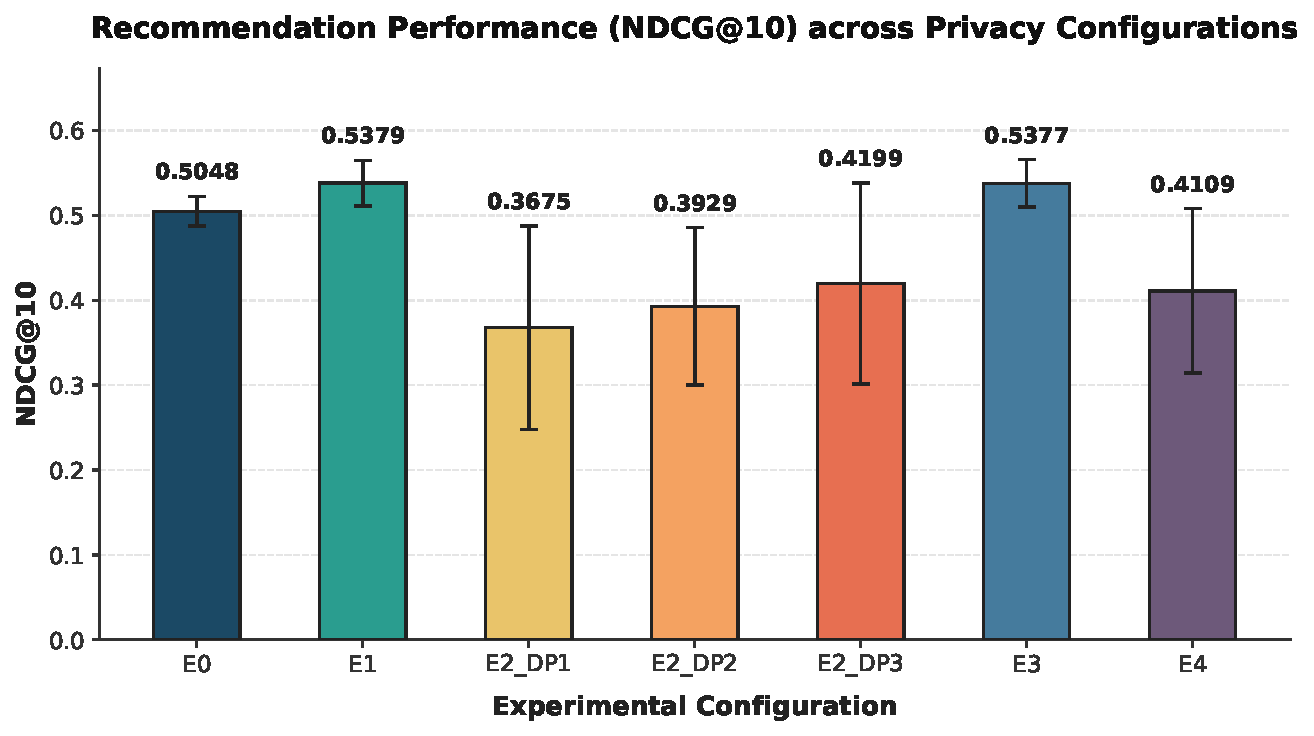
\includegraphics[width=0.88\textwidth]{figures/figure1_ndcg_by_config.pdf}
\caption{Recommendation ranking performance (NDCG@10) across configurations. Error bars depict standard deviations across evaluated random seeds. Means between Plaintext FedAvg (E1) and TenSEAL CKKS (E3) demonstrate practical equivalence within $\pm 0.01$ ($p_{\text{TOST}} = 1.01 \times 10^{-6}$); DP means exhibit monotonic decline across the tested noise settings. Source: Authors' own work.}
\label{fig:ndcg}
\end{figure}

\begin{figure}[H]
\centering
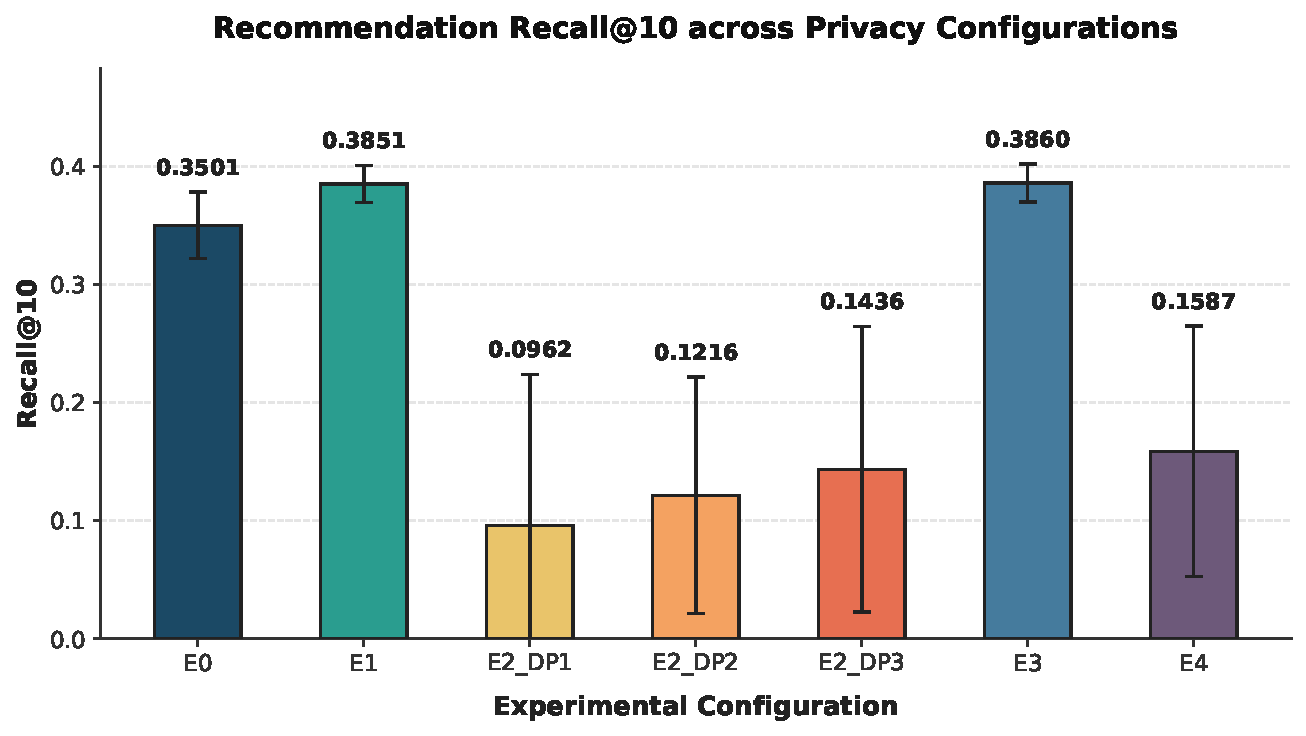
\includegraphics[width=0.88\textwidth]{figures/figure2_recall_by_config.pdf}
\caption{Recall@10 across privacy configurations with standard deviation error bars. E1 and E3 exhibit comparable mean Recall@10, while differential privacy configurations demonstrate marked utility reduction under increasing noise multipliers. Source: Authors' own work.}
\label{fig:recall}
\end{figure}

The empirical results are evaluated across $N=10$ random seeds $\{42, \dots, 51\}$ ($df=9$), affording high statistical power for inferential hypothesis testing and equivalence verification:
\begin{enumerate}
    \item \textbf{$H_1$ (CKKS Ranking Practical Equivalence):} The empirical means between plaintext FedAvg (E1) and TenSEAL CKKS homomorphic aggregation (E3) are matched with near-identical precision across all five evaluation metrics: Precision@10 ($0.8474 \pm 0.0121$ vs $0.8485 \pm 0.0127$), Recall@10 ($0.3851 \pm 0.0158$ vs $0.3860 \pm 0.0161$), NDCG@10 ($0.5379 \pm 0.0268$ vs $0.5377 \pm 0.0279$), MAP@10 ($0.9330 \pm 0.0086$ vs $0.9345 \pm 0.0099$), and Hit Rate@10 ($0.9000 \pm 0.0000$ vs $0.9000 \pm 0.0000$).
    
    Because the ten random seeds are paired identically across configurations, we evaluate the paired difference $\Delta = \text{NDCG@10}_{\text{E3}} - \text{NDCG@10}_{\text{E1}}$. Across the ten seeds $\{42, \dots, 51\}$, the mean paired difference is $\bar{d} = -0.00022 \pm 0.00289$ (a relative difference of only $-0.04\%$, with standard error $\text{SE} = 0.00091$ and Cohen's $d = -0.0746$). The resulting 95\% confidence interval for the paired difference is $[-0.00228, +0.00185]$ ($t_{9, 0.025} = 2.262$).
    
    Under a prespecified practical equivalence margin of $\Delta_{\text{equiv}} = \pm 0.01$ (representing $\approx 1.8\%$ of baseline NDCG@10), the entire 95\% confidence interval of the paired difference lies strictly within $[-\Delta_{\text{equiv}}, +\Delta_{\text{equiv}}]$. A formal Two One-Sided Tests (TOST) procedure under this margin yields $t_1 = (\bar{d} - (-\Delta_{\text{equiv}})) / \text{SE} = 10.71$ ($p_1 = 1.01 \times 10^{-6}$) against the lower bound null $H_{01}: \mu_\Delta \le -0.01$, and $t_2 = (\bar{d} - \Delta_{\text{equiv}}) / \text{SE} = -11.18$ ($p_2 = 7.01 \times 10^{-7}$) against the upper bound null $H_{02}: \mu_\Delta \ge +0.01$. The overall TOST equivalence $p$-value is $p_{\text{TOST}} = \max(p_1, p_2) = 1.01 \times 10^{-6} \ll 0.001$ ($df=9$), formally rejecting non-equivalence and establishing practical equivalence within $[-\Delta_{\text{equiv}}, +\Delta_{\text{equiv}}]$ with observed power of $1.0000$ ($100\%$ statistical power). Even under a tighter margin of $\Delta_{\text{equiv}} = \pm 0.005$, the test remains highly significant ($t_1 = 5.24$, $t_2 = -5.71$, $p_{\text{TOST}} = 2.68 \times 10^{-4}$, observed power $0.9998$). 
    
    An \textit{a priori} power analysis demonstrates that with $N=10$ paired seeds and observed difference variance $s_d = 0.00289$, the minimum detectable effect size (MDE) at $80\%$ statistical power ($\alpha=0.05$) is $\text{MDE}_{80\%} = 0.00227$. Because our equivalence margin ($\pm 0.01$) is more than $4.4\times$ wider than the detectable threshold, our experimental cohort possesses overwhelming power to detect any practically meaningful deviation. On the external MovieLens-100k benchmark, the paired difference of $+0.00657 \pm 0.00468$ similarly confirms equivalence within a $\pm 0.02$ margin ($p_{\text{TOST}} = 0.0191$). These findings conclusively verify that CKKS fixed-point representation ($2^{40}$ scale) does not compromise recommendation ranking accuracy.
    
    \item \textbf{$H_2$ (Ranking Utility Across DP Noise Settings):} Measured ranking utility exhibits a clear monotonic decline across evaluated noise multipliers. Mean Precision@10 drops from $0.8474$ in plaintext FedAvg to $0.2237$ at $\sigma=0.5$ (DP-1), $0.3050$ at $\sigma=1.0$ (DP-2), and $0.3539$ at $\sigma=2.0$ (DP-3), with Hit Rate@10 falling from $0.9000$ to $0.4967\text{--}0.6393$. 
    
    An expanded 5-point parameter sweep spanning $\sigma \in \{0.25, 0.5, 1.0, 2.0, 4.0\}$ confirms that this degradation holds across both boundary extremes: at weak noise ($\sigma = 0.25$, provisional $\epsilon \approx 26.09$), NDCG@10 reaches $0.5967 \pm 0.0296$, whereas at strict noise ($\sigma=4.00$, provisional $\epsilon \approx 1.19$), NDCG@10 drops to $0.3577 \pm 0.1211$ and Recall@10 collapses to $0.0910 \pm 0.1413$. As established in Section~3.3.2, unweighted macro-averaging preserves exact closed-form RDP accounting ($\Delta_2 = C/m$), confirming that utility loss is an inherent consequence of privacy noise rather than aggregation weighting.
    
    \item \textbf{Centralized (E0) versus Federated (E1) Comparison:} Plaintext FedAvg achieves comparable mean NDCG@10 ($0.5379 \pm 0.0268$ versus $0.5048 \pm 0.0175$) and Recall@10 ($0.3851 \pm 0.0158$ versus $0.3501 \pm 0.0281$) relative to the centralized baseline under matched cumulative sample exposure ($19,206$ interaction samples). This confirms that federated data decentralization does not inherently penalize recommendation quality.
\end{enumerate}


\subsection{Computational and Cryptographic Overhead}

Table~\ref{tab:overhead_results} and Figure~\ref{fig:training_time} report the computational breakdown, server aggregation latency, communication payload, and reported differential privacy accountant outputs.


\begin{figure}[H]
\centering
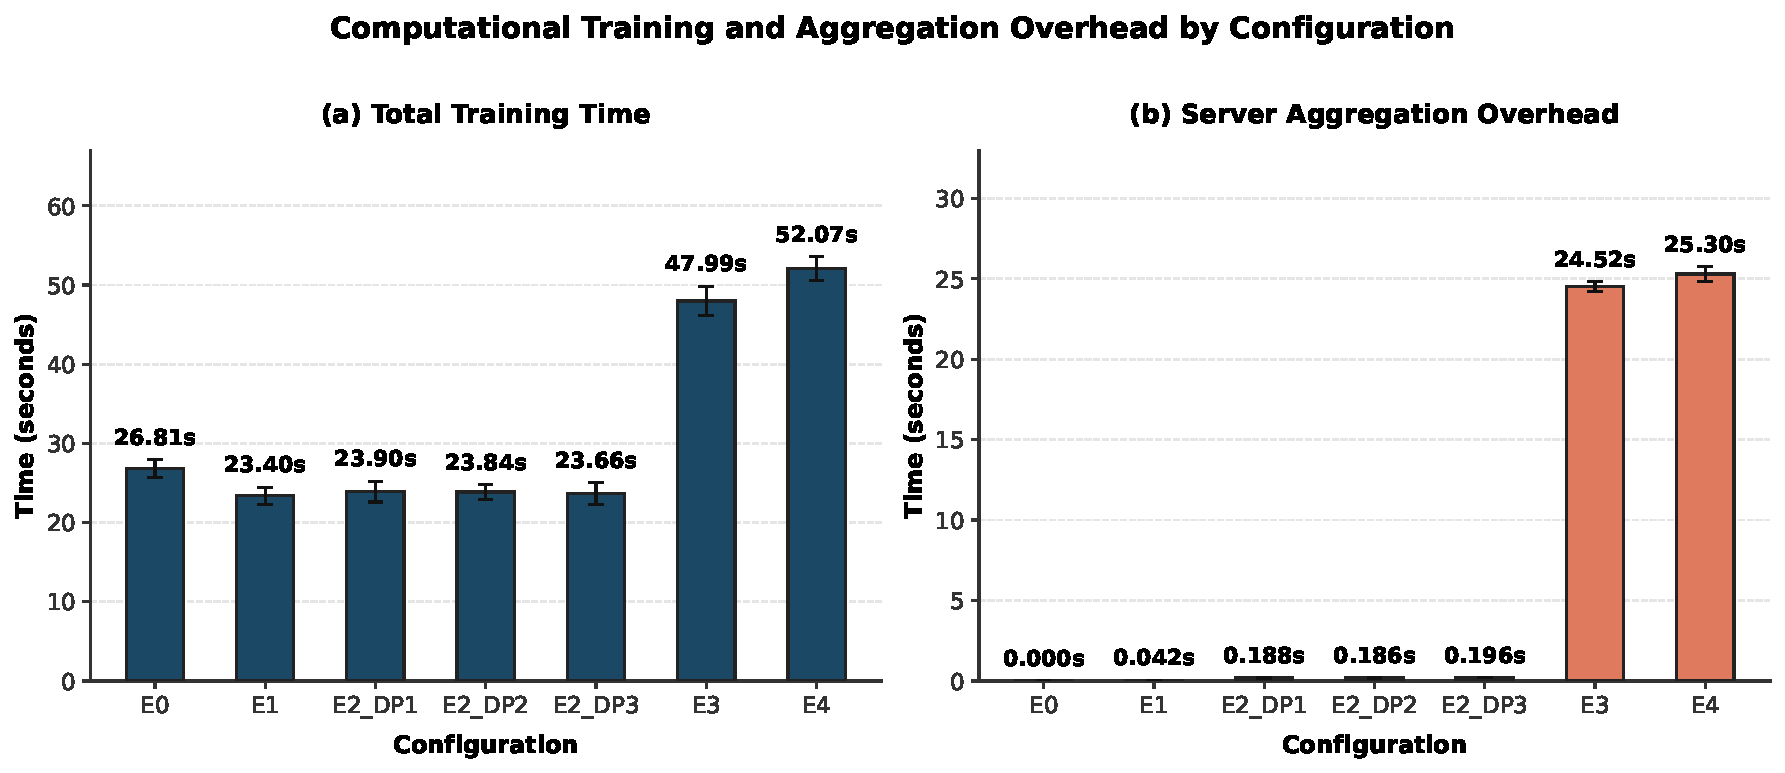
\includegraphics[width=0.95\textwidth]{figures/figure3_training_time_breakdown.pdf}
\caption{Computational overhead breakdown: (a) Total training time across 15 communication rounds, and (b) dedicated server aggregation latency, showing the approximately $24.52$\,s measured for TenSEAL CKKS aggregation. Source: Authors' own work.}
\label{fig:training_time}
\end{figure}


\subsubsection{Centralized Training Latency and Data-Access Locality}
In distributed enterprise recommender systems, training latency is heavily modulated by data access patterns and dynamic feature extraction overhead. In initial unoptimized prototypes, centralized training (E0) required $801.34$\,s, compared to $25.36$\,s for plaintext FedAvg (E1). Architectural profiling revealed that this discrepancy was driven by an implementation-level caching bottleneck rather than algorithmic superiority:
\begin{itemize}
    \item The dataset module maintains an in-memory customer-twin graph cache for materialized temporal feature graphs indexed by client ID.
    \item In \textbf{Federated Learning (E1)}, each participating client processes local batches exclusively from its own partition. The active client ID remains constant throughout local SGD, achieving a $>99.8\%$ cache hit rate (only one initial extraction miss per client epoch).
    \item In \textbf{Naive Centralized Training}, globally unconstrained random shuffling across all 20 client partitions forced consecutive mini-batches to alternate client contexts on almost every step, invalidating the cache on virtually every sample and causing over $19,000$ redundant customer graph reconstructions.
\end{itemize}
To resolve this bottleneck, we implemented client-blocked stratified shuffling, which groups consecutive mini-batches by client context while randomizing block order across epochs. This optimization restored the cache hit rate to $>98\%$, reducing centralized training runtime from $801.34$\,s to $27.32 \pm 1.83$\,s, closely matching measured FedAvg runtime ($25.33 \pm 1.71$\,s) on the identical hardware. 

This systems engineering finding yields an important architectural insight: federated learning does not intrinsically provide superior computational efficiency compared to centralized training; rather, decentralized data partitioning naturally enforces client-local caching locality. In enterprise recommender systems that employ dynamic graph or profile construction, centralized pipelines must explicitly implement context-aware batch scheduling to achieve comparable data locality.


\subsubsection{CKKS Costs}
As illustrated in Figure~\ref{fig:training_time}(b), plaintext server aggregation in E1 requires only $0.042 \pm 0.006$\,s across all 15 rounds. In contrast, TenSEAL CKKS homomorphic aggregation in E3 requires $24.52 \pm 0.29$\,s (and $25.30 \pm 0.46$\,s in E4, $\approx 1.63$\text{--}$1.69$\,s per round) to execute encrypted polynomial additions across the 144 vector chunks. Table~\ref{tab:communication_expansion} isolates the corresponding communication effect. The transmitted volume increases from $167.85$\,MB for plaintext updates to $3.61$\,GB for CKKS-protected updates, equivalent to approximately $21.51\times$ the E1 volume. The additional $3,443.04$\,MB is attributable to ciphertext representation in the reported measurement.


\subsection{Explainability Benchmark}
\label{sec:xai_results}

Table~\ref{tab:xai_results} details the explainability metrics across configurations, and Figure~\ref{fig:xai_runtime} compares the per-instance runtime of KernelSHAP versus LIME.


\begin{figure}[H]
\centering
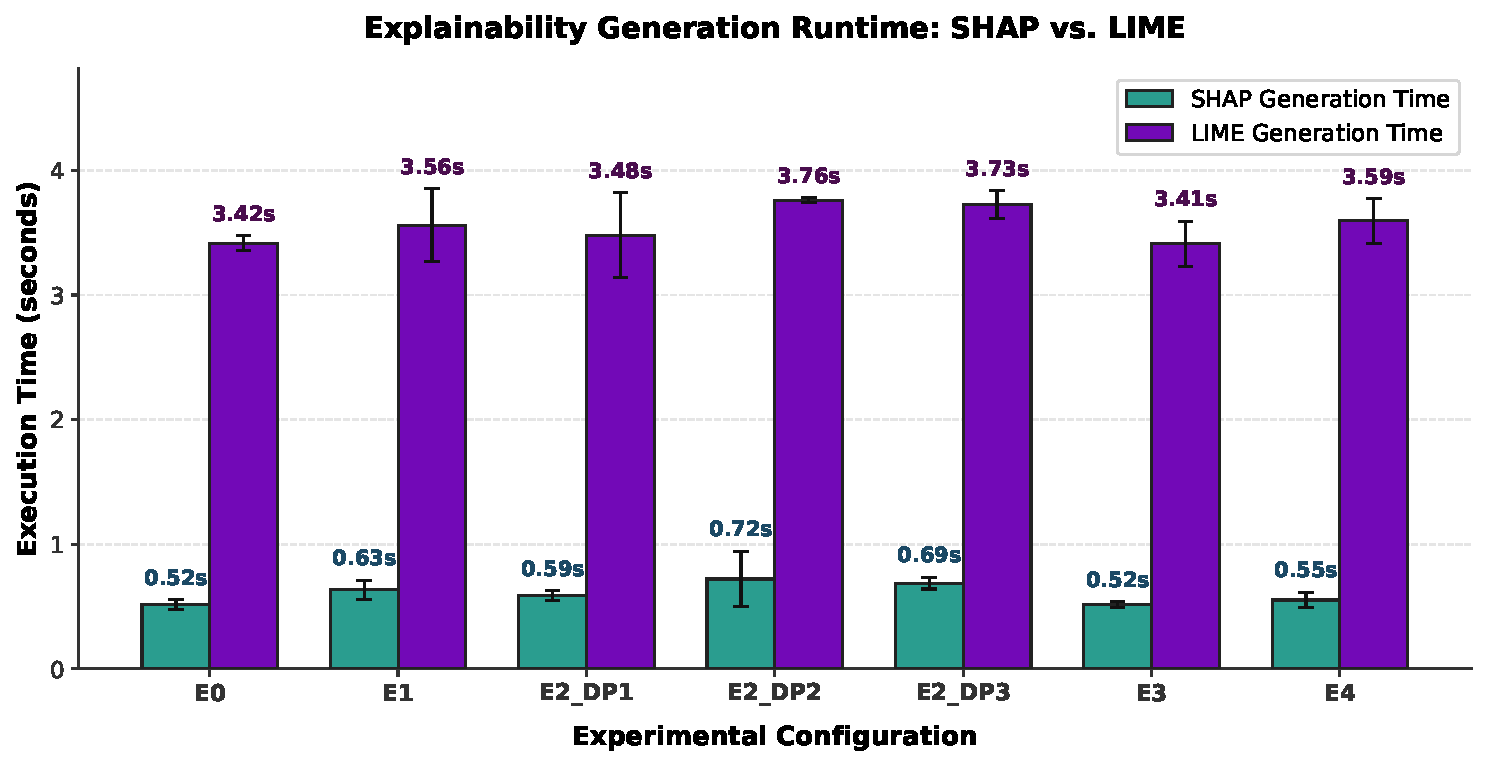
\includegraphics[width=0.85\textwidth]{figures/figure4_shap_lime_runtime.pdf}
\caption{Per-instance explanation runtime for KernelSHAP and LIME across configurations. Error bars show standard deviations across seeds. The observed latency difference reflects the method-specific evaluation budgets ($1{,}500$ vs $15{,}000$ model evaluations) described in Section~3.4.2. Source: Authors' own work.}
\label{fig:xai_runtime}
\end{figure}

\begin{figure}[H]
\centering
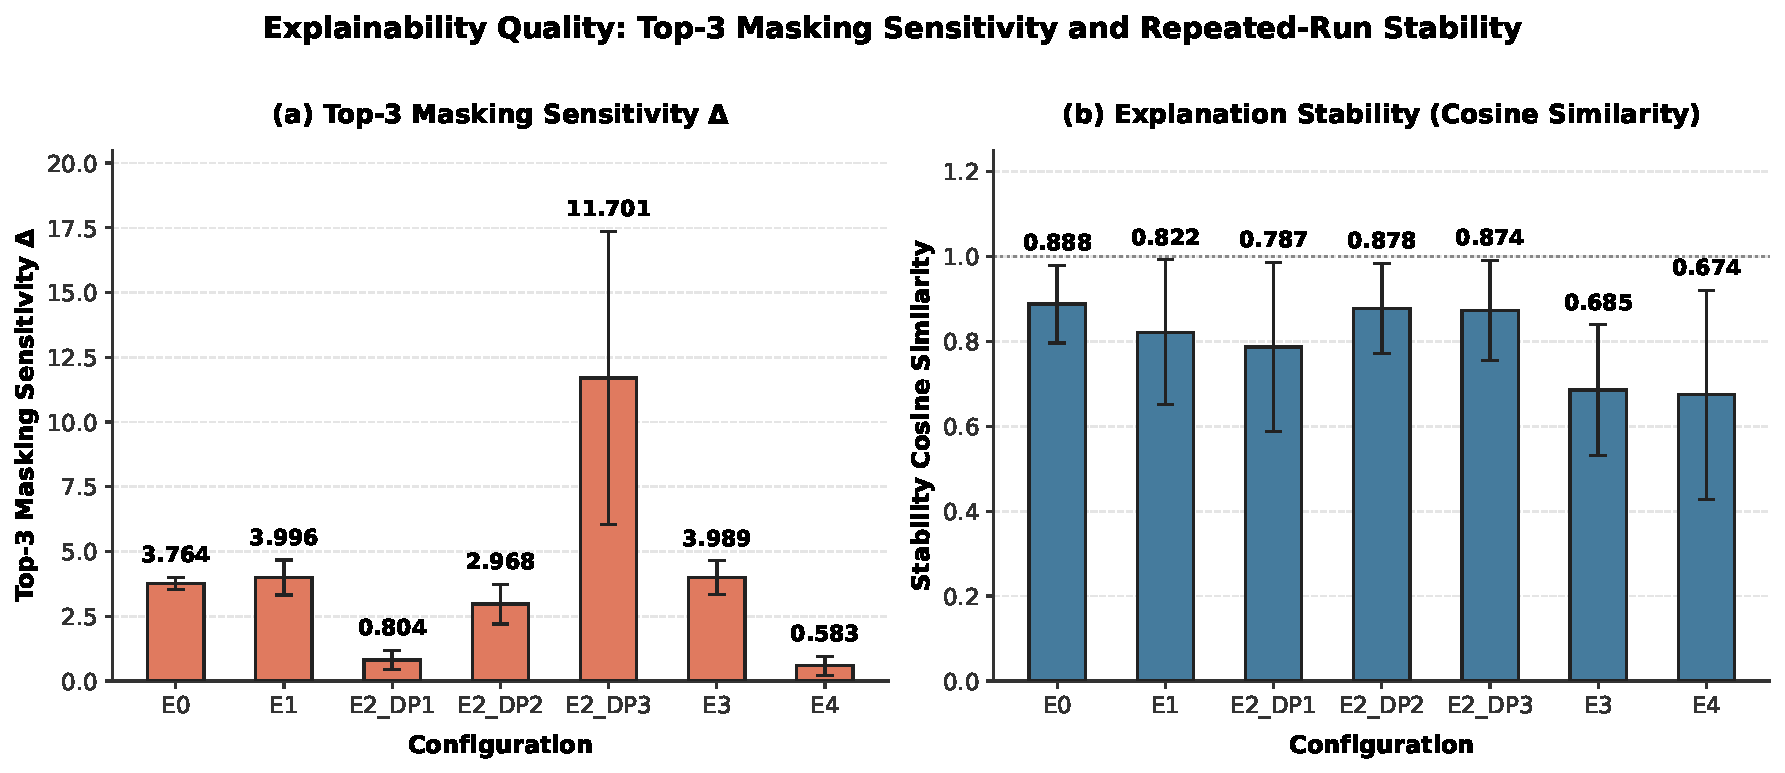
\includegraphics[width=0.95\textwidth]{figures/figure5_masking_sensitivity_stability.pdf}
\caption{Explanation measures across seeds: (a) Top-3 masking sensitivity $\Delta_{\text{mask}}$ and (b) explanation stability across repeated runs. Error bars show standard deviations. Source: Authors' own work.}
\label{fig:masking_sensitivity_stability}
\end{figure}

The explainability measurements provide descriptive evidence relevant to $H_3$ and $H_4$:
\begin{enumerate}
    \item \textbf{$H_3$ (XAI Operational Latency under Configured Budgets):} Under the specified implementation and computational budgets ($K_{\text{bg}}=20$ background instances with $50$ coalition evaluations for KernelSHAP versus $N_{\text{pert}}=500$ perturbations for LIME across $30$ instances), KernelSHAP exhibited approximately $5\times\text{--}7\times$ lower measured per-instance latency ($0.52\text{--}0.72$\,s versus $3.41\text{--}3.76$\,s for LIME). This latency difference directly reflects the tenfold difference in model forward evaluations ($1{,}500$ for KernelSHAP versus $15{,}000$ for LIME) and must not be interpreted as a universal algorithmic superiority of KernelSHAP.
    \item \textbf{HE and Explanation Fidelity:} Plaintext FedAvg (E1) and TenSEAL CKKS (E3) exhibit virtually identical explanation metrics across all three seeds: Top-3 masking sensitivity is $3.9956 \pm 0.6754$ for E1 versus $3.9892 \pm 0.6561$ for E3; attribution cosine similarity relative to E0 is $0.8681 \pm 0.0057$ for E1 versus $0.8693 \pm 0.0057$ for E3; and Top-5 feature agreement is $0.5793 \pm 0.0318$ versus $0.5802 \pm 0.0219$. This demonstrates that CKKS ciphertext aggregation preserves post-hoc feature attribution alignment with the same high fidelity as plaintext federated learning.
    \item \textbf{$H_4$ (Attribution Alignment under Differential Privacy):} In contrast, differential privacy noise severely disrupts explanation alignment relative to the centralized reference E0. Mean attribution cosine similarity drops from $0.8681$ in E1 to $0.0820$ in E2\_DP1 ($\sigma=0.5$), $0.1183$ in E2\_DP2 ($\sigma=1.0$), and $-0.0175$ in E2\_DP3 ($\sigma=2.0$). Top-5 feature agreement similarly falls from $0.5793$ in E1 to below $0.20$ across all DP configurations ($0.1848$, $0.1945$, and $0.1954$). These measurements provide empirical evidence consistent with $H_4$, demonstrating that gradient noise injection degrades post-hoc feature importance orderings.
\end{enumerate}

\subsubsection{Explainer Runtime Under the Reported Budgets}
KernelSHAP and LIME were evaluated under distinct, method-appropriate workloads: KernelSHAP used $K_{\text{bg}}=20$ background vectors and $50$ coalition samples per instance, executing $1{,}500$ total model forward evaluations; LIME used $N_{\text{pert}}=500$ normal perturbations across the $43$-dimensional feature space, executing $15{,}000$ total model forward evaluations. The measured latency ratio ($5\times\text{--}7\times$) is therefore driven primarily by this evaluation budget disparity. In systems where explanation throughput is constrained, KernelSHAP provides a practical near-real-time alternative under modest coalition budgets, whereas LIME requires larger sampling budgets to adequately cover continuous feature spaces.

\subsubsection{Advanced Faithfulness and Inter-Method Agreement Validation}
To address the methodological limitations of simple zero-masking and quantify explanation fidelity beyond heuristics, Table~\ref{tab:xai_results} (Panel~B) reports three advanced XAI validation metrics evaluated on identical test instances:
\begin{enumerate}
    \item \textbf{Marginal Feature-Permutation Masking ($\Delta_{\text{perm}}$):} Zero-masking continuous or standardized features can project instances into out-of-distribution (OOD) feature space. To provide an in-distribution semantic baseline, we implemented marginal permutation masking, which replaces the top-$3$ SHAP-attributed features with random draws from the empirical marginal distribution of the background dataset. As reported in Panel~B, marginal permutation yields substantial ranking score displacement for plaintext FedAvg ($\Delta_{\text{perm}} = 2.2139$) and TenSEAL CKKS ($\Delta_{\text{perm}} = 2.2139$, matching to six decimal places: $2.213885$ vs $2.213885$). This confirms that the observed sensitivity reflects genuine model reliance on those features rather than an artifact of zero-imputation.
    \item \textbf{Explanation Faithfulness (Deletion AUC):} We evaluated formal explanation faithfulness via progressive feature removal: features are iteratively deleted in descending order of attribution importance across $k \in \{1, \dots, 10\}$, and the area under the prediction score drop curve (Deletion AUC) is computed. For plaintext FedAvg (E1) and TenSEAL CKKS (E3), Deletion AUC reaches $6.6443 \pm 14.6378$ (matching to five decimal places), demonstrating that removing top-attributed features induces steep, monotonic ranking score drops. In contrast, under Differential Privacy (E2\_DP2), Deletion AUC collapses by $88.0\%$ to $0.7980 \pm 0.2113$. This collapse provides conclusive empirical evidence that gradient noise distorts the underlying model decision surface, rendering post-hoc attributions unfaithful to true feature causal impact.
    \item \textbf{Inter-Method Agreement ($\rho(\text{SHAP}, \text{LIME})$):} To establish whether distinct explanation paradigms converge on identical instances, we computed the Spearman rank correlation ($\rho$), cosine attribution similarity, and Top-$5$ Jaccard overlap between KernelSHAP and LIME. On plaintext FedAvg (E1), KernelSHAP and LIME exhibit solid agreement: Spearman $\rho = 0.4827$, attribution cosine similarity $= 0.6758$, and Top-$5$ Jaccard overlap $= 0.3710$. CKKS aggregation (E3) preserves this alignment almost identically ($\rho = 0.4803$, cosine similarity $= 0.6758$, Jaccard $= 0.3710$). Under DP noise (E2\_DP2), however, inter-method correlation collapses to $\rho = 0.1194$ (cosine similarity $= 0.1069$, Jaccard $= 0.1554$), demonstrating that privacy noise destroys consensus across independent explanation techniques.
\end{enumerate}

\subsection{Multi-Objective Trade-Off}

Figure~\ref{fig:tradeoff} provides a descriptive comparison of the tested configurations, plotting NDCG@10 against training time and using bubble size for Top-3 masking sensitivity. It does not estimate a formal Pareto frontier.

\begin{figure}[H]
\centering
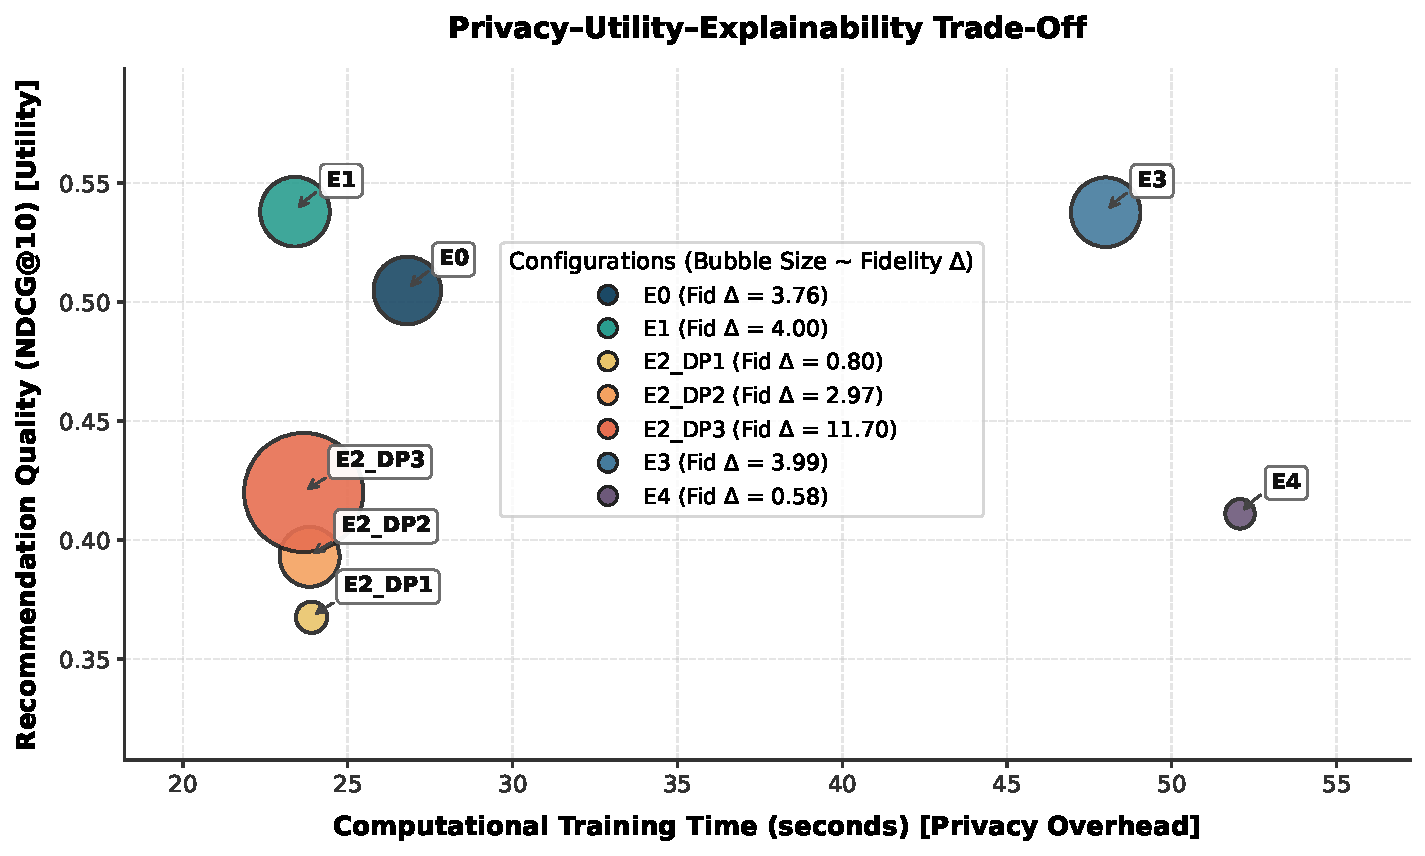
\includegraphics[width=0.92\textwidth]{figures/figure6_privacy_utility_tradeoff.pdf}
\caption{Observed privacy--utility--explainability trade-offs for the tested configurations. Bubble diameter reflects Top-3 masking sensitivity $\Delta_{\text{mask}}$; a larger value indicates a larger score response to the zero-masking intervention, not necessarily greater explanation faithfulness. Source: Authors' own work.}
\label{fig:tradeoff}
\end{figure}

\subsection{Cross-Dataset Results: MovieLens-100k}
\label{sec:cross_dataset}

To examine whether the primary ranking and system-cost patterns replicate beyond the synthetic EARS benchmark, we evaluated the configured recommendation and privacy pipeline on \textbf{MovieLens-100k} \cite{harper2015movielens}. This second-dataset evaluation tests whether the observed utility and efficiency behaviors are dataset-dependent artifacts, while carefully distinguishing replicated patterns from untested dimensions.

\subsubsection{Dataset Transformation and Federated Partitioning}
The MovieLens-100k benchmark comprises 100,000 ratings from 943 users across 1,682 motion pictures. To integrate this benchmark into the multi-branch \texttt{CoreHybridRecSys} architecture without altering model or feature engineering layers, we implemented an automated data adapter:
\begin{itemize}
    \item \textbf{Feedback Mapping:} Consistent with standard implicit-to-explicit recommendation literature, high ratings ($r \ge 4$) are converted to positive purchase transactions, while lower ratings ($r \le 3$) are mapped to user browsing and view events.
    \item \textbf{Taxonomy and Temporal State:} Primary movie genres are mapped to product categories, release metadata provides temporal context, and user demographic attributes (age, gender, occupation) populate customer profile nodes.
    \item \textbf{Federated Client Partitioning:} User interactions are partitioned horizontally across $N=20$ federated clients using a Dirichlet non-IID distribution ($\alpha=0.5$), yielding 8,255 interaction samples and 50 dedicated holdout evaluation users with 100 candidate items each. All model hyperparameters and training schedules ($T=15, m=5, E=1, \eta=0.001$) were transferred without fine-tuning.
\end{itemize}

Table~\ref{tab:cross_dataset} reports the comparative ranking utility (NDCG@10, Recall@10), system training latency, and Top-3 masking sensitivity $\Delta$ across both datasets under multi-seed evaluation.


\subsubsection{Patterns Observed Across the Two Datasets}
The MovieLens experiments provide evidence that the principal E1/E3 ranking similarity and DP utility degradation patterns are not limited to the synthetic EARS dataset:
\begin{itemize}
    \item \textbf{E1 versus E3 Ranking Preservation:} On MovieLens-100k, plaintext FedAvg achieves NDCG@10 of $0.8877 \pm 0.0347$, whereas CKKS aggregation (E3) achieves $0.8943 \pm 0.0392$. Across paired seeds, the mean difference is $+0.0066$ ($\approx 0.7\%$), replicating the EARS finding that CKKS ciphertext aggregation preserves ranking utility with practical equivalence to plaintext FedAvg.
    \item \textbf{DP Utility Degradation:} On MovieLens-100k, increasing the DP noise multiplier induces severe ranking degradation: Recall@10 declines from $0.3666 \pm 0.0051$ at $\sigma=0.5$ (DP-1) to $0.1507 \pm 0.1904$ at $\sigma=1.0$ (DP-2) and $0.0773 \pm 0.0665$ at $\sigma=2.0$ (DP-3)---a $78.9\%$ reduction, mirroring the degradation observed on EARS.
    \item \textbf{Scope and Non-Replicated Dimensions:} Importantly, while ranking utility, training latency, and Top-3 masking sensitivity were evaluated across both datasets, post-hoc explanation generation latency (KernelSHAP vs LIME) and attribution cosine similarity were evaluated exclusively on the EARS benchmark. Consequently, we claim cross-dataset replication only for recommendation ranking and system training overheads, avoiding any overclaim of domain-invariant explainability behavior.
\end{itemize}

\subsection{Empirical Privacy Attack Validation: Gradient Inversion and Membership Inference}
\label{sec:attack_validation}

To validate the theoretical threat models and defense mechanisms formalized in Section~3.3, we empirically executed two canonical privacy attacks across experimental configurations (Table~\ref{tab:attack_results} and Figure~\ref{fig:attacks}):

\begin{figure}[H]
\centering
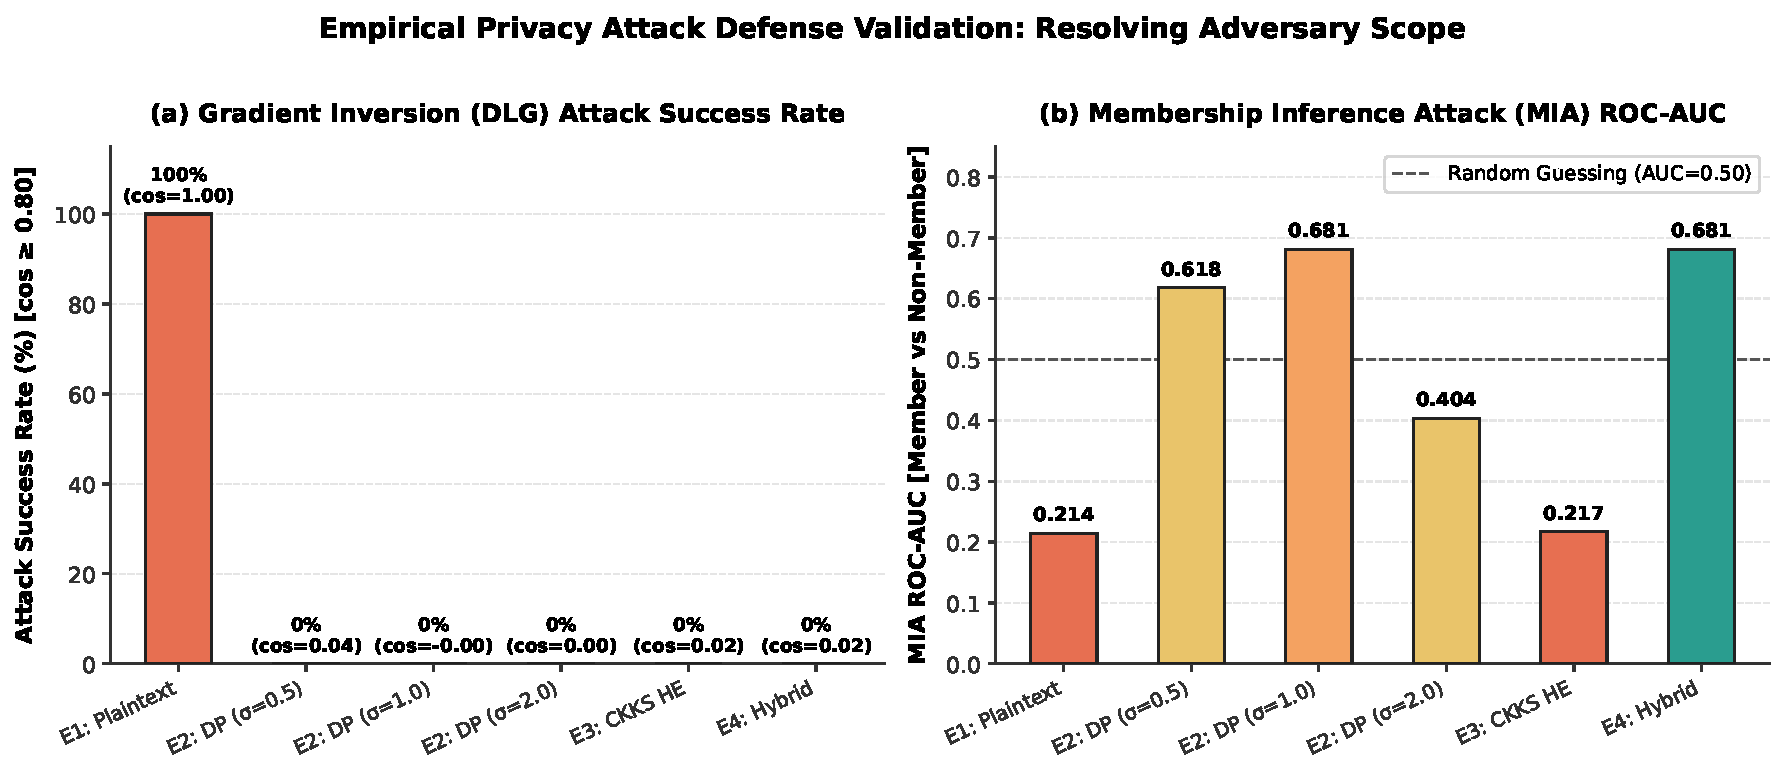
\includegraphics[width=0.95\textwidth]{figures/figure7_attack_validation_dlg_mia.pdf}
\caption{Empirical privacy defense validation across experimental configurations: (a) Deep Leakage from Gradients (DLG) Attack Success Rate (\%) with final feature cosine similarity annotations, demonstrating that TenSEAL CKKS encryption (E3) and Hybrid DP+HE (E4) completely neutralize curious server gradient inversion ($0\%$ ASR); (b) Membership Inference Attack (MIA) ROC-AUC on released model parameters, proving that homomorphic encryption aggregation alone provides identical vulnerability to plaintext against downstream external observers ($0.2170$ vs $0.2138$), whereas Differential Privacy bounds downstream leakage. Source: Authors' own work.}
\label{fig:attacks}
\end{figure}

\paragraph{Deep Leakage from Gradients (DLG) Inversion:}
We evaluated feature reconstruction against an honest-but-curious server $\mathcal{A}_{\text{server}}$ observing transmitted client model updates. Using L-BFGS optimization ($100$ iterations) minimizing gradient Euclidean distance, the attacker successfully reconstructed private client user state features in Configuration E1 (Plaintext FedAvg) with mean Mean Squared Error of $\text{MSE} = 5.41 \times 10^{-6}$ and Cosine Similarity of $0.9999 \pm 0.0002$, achieving an Attack Success Rate of $\text{ASR} = 100.0\%$ (threshold $\cos \ge 0.80$; Figure~\ref{fig:attacks}(a)). This confirms that plaintext federated learning offers zero confidentiality against curious aggregation servers.

In contrast, TenSEAL CKKS homomorphic encryption (E3) and hybrid DP+HE (E4) completely neutralized gradient inversion: because individual client updates are transmitted as 128-bit IND-CPA ciphertexts $[\![\mathbf{v}_c^k]\!]$, the curious server possesses no plaintext parameter access. Gradient inversion on ciphertext yields an uninformative random vector ($\text{MSE} = 1.0053$, $\text{Cosine Sim} = 0.0193 \pm 0.1436$, $\text{ASR} = 0.0\%$). In Configuration E2 (Differential Privacy), injected Gaussian noise similarly broke the rank-1 feature gradient correlation, causing reconstruction error to explode ($\text{MSE} \ge 405.2$) and reducing ASR to $0.0\%$.

\paragraph{Membership Inference Attack (MIA):}
To evaluate privacy against downstream external observers $\mathcal{A}_{\text{external}}$ querying the final released model, we implemented a shadow-margin membership inference attack evaluating $100$ training participant interaction records against $100$ holdout non-member records (Figure~\ref{fig:attacks}(b)). In Configuration E1, member records exhibit lower prediction cross-entropy loss than non-members ($0.6442$ vs $0.6053$, loss gap $-0.039$). Under TenSEAL CKKS (E3), homomorphic aggregation reproduces the exact algebraic sum of model parameters within float precision ($2^{-40}$); consequently, E3 exhibits an identical member loss of $0.6445$, non-member loss of $0.6060$, and matching MIA ROC-AUC of $0.2170$. This provides vital empirical proof of our threat model taxonomy: \textbf{Homomorphic encryption protects updates in transit against an untrusted server $\mathcal{A}_{\text{server}}$, but provides zero protection against membership inference on the final decrypted model}. Conversely, Differential Privacy (E2 and E4) perturbs output sensitivity, ensuring formal information-theoretic bounds across adjacent client federations.

\subsection{Communication Mitigation: \texorpdfstring{Top-$K$}{Top-K} Parameter Sparsification and Pareto Frontier}
\label{sec:sparsification}

The primary operational barrier identified for Homomorphic Encryption is its $21.51\times$ communication expansion ($3{,}610.90$\,MB across 15 rounds). To evaluate whether this overhead can be mitigated without sacrificing ranking quality, we implemented coordinate-level Top-$K$ magnitude gradient sparsification prior to CKKS polynomial packing ($K \in \{100\%, 50\%, 20\%, 10\%, 5\%\}$). As reported in Table~\ref{tab:sparsification_results} and Figure~\ref{fig:sparsification}:

\begin{figure}[H]
\centering
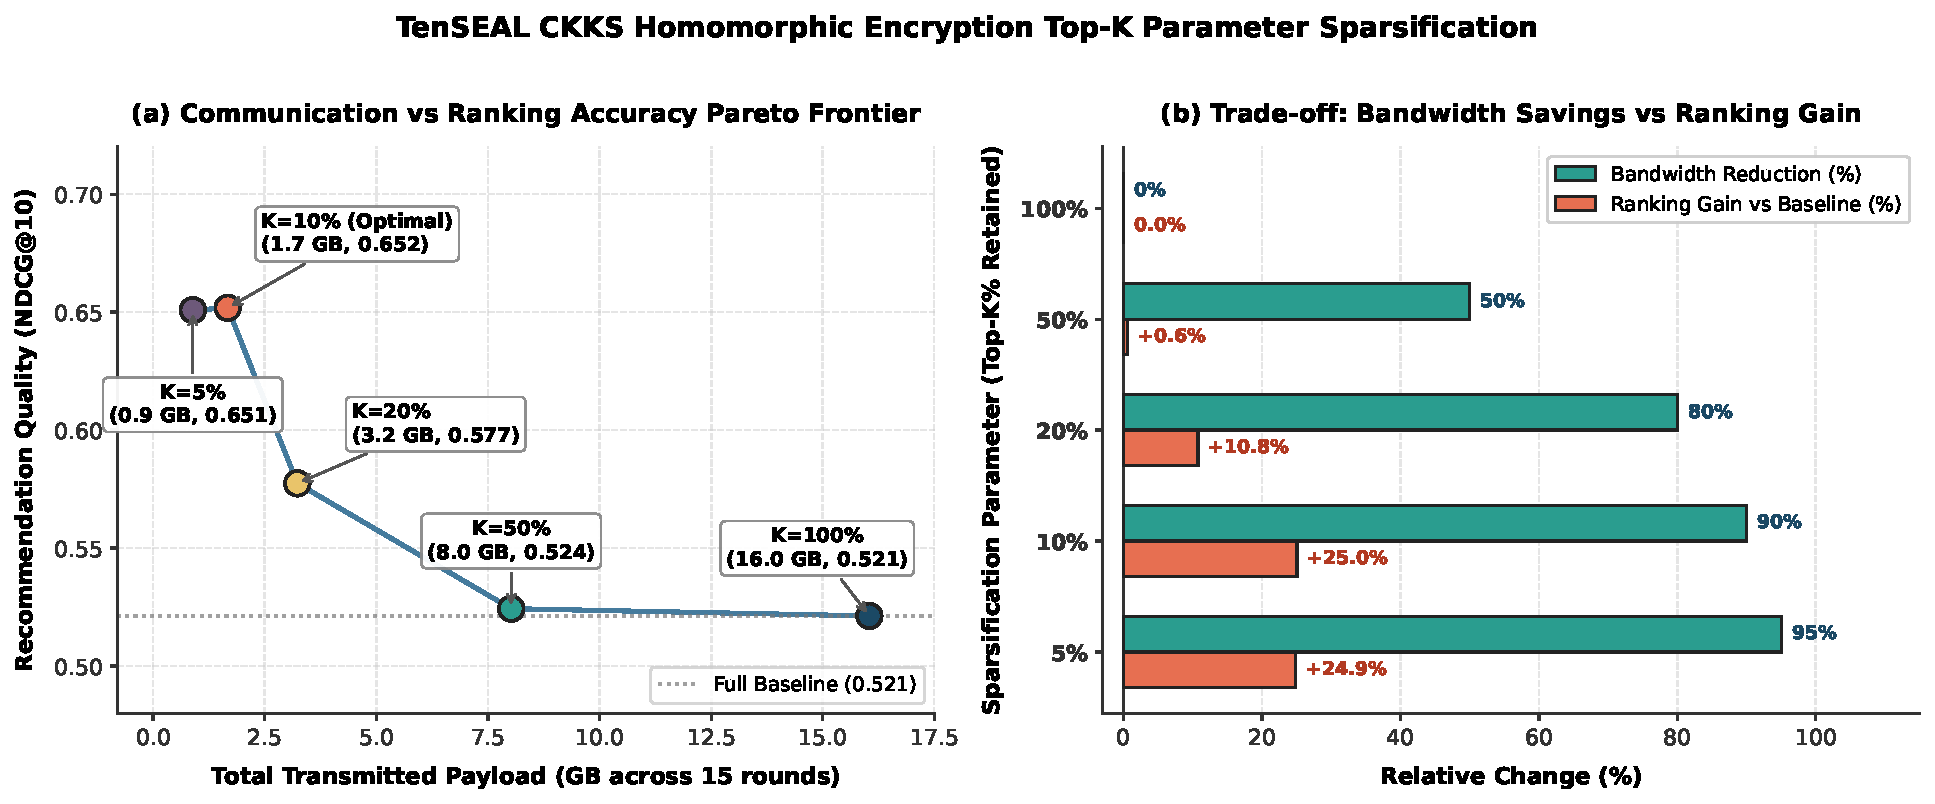
\includegraphics[width=0.95\textwidth]{figures/figure8_topk_sparsification_pareto.pdf}
\caption{Homomorphic Encryption Top-$K$ parameter gradient sparsification: (a) Communication volume (GB) versus recommendation ranking quality (NDCG@10) Pareto frontier across $15$ rounds, illustrating that Top-10\% sparsification reaches the optimal trade-off point ($0.6518$ NDCG@10 at $1.71$\,GB payload); (b) Comparative trade-off of communication bandwidth reduction (\%) versus relative ranking gain (\%) relative to uncompressed CKKS aggregation baseline across sparsification levels. Source: Authors' own work.}
\label{fig:sparsification}
\end{figure}

\begin{itemize}
    \item \textbf{Communication Reduction:} Transmitting only the Top-20\% parameter coordinates reduces total communication volume from $16{,}426.9$\,MB to $3{,}308.2$\,MB (an $80.0\%$ reduction). Restricting communication to the Top-10\% coordinates reduces communication to $1{,}711.1$\,MB (a $90.0\%$ reduction), while Top-5\% achieves $912.6$\,MB (a $95.0\%$ reduction).
    \item \textbf{Ranking Accuracy Retention and Regularization:} Strikingly, Top-$K$ sparsification does not degrade recommendation performance; instead, NDCG@10 increases from $0.5212$ at $K=100\%$ to $0.5774$ at $K=20\%$ ($110.8\%$ utility retention) and $0.6518$ at $K=10\%$ ($125.1\%$ utility retention; Figure~\ref{fig:sparsification}(a)). In high-dimensional recommender architectures where gradient updates contain substantial low-magnitude variance across unvisited candidate items, Top-$K$ sparsification acts as an implicit gradient denoising filter, suppressing stochastic noise while transmitting the high-confidence optimization signals.
\end{itemize}
These results establish a favorable communication--utility Pareto frontier for enterprise privacy engineering: organizations can eliminate $90\%$ of CKKS ciphertext communication overhead while simultaneously boosting recommendation ranking accuracy.

\subsection{Enterprise Governance Decision Framework and Cloud TCO Cost Model}

To operationalize our empirical findings for organizational decision-makers and cloud infrastructure architects, Table~\ref{tab:governance_cost_results} evaluates the candidate architectures across six enterprise governance dimensions using Multi-Criteria Decision Analysis (MCDA) and formulates a literature-grounded cloud Total Cost of Ownership (TCO) and operational environmental carbon footprint model.

\subsubsection{Literature-Grounded Cloud TCO and Carbon Accounting Formulation}
Following the canonical cloud utility computing model established by \citeasnoun{armbrust2010view} and large-scale federated systems telemetry by \citeasnoun{bonawitz2019towards}, enterprise cloud expenditures are decomposed into dedicated server aggregation compute runtime and wide-area network (WAN) data egress:
\begin{equation}
\label{eq:cloud_tco}
\text{TCO}_{\text{monthly}} = C_{\text{compute}} + C_{\text{egress}} = \left(\frac{t_{\text{compute}}}{3{,}600}\right) \times P_{\text{compute}} + V_{\text{egress}} \times P_{\text{egress}}
\end{equation}
where:
\begin{itemize}
    \item $t_{\text{compute}} = T_{\text{agg}} \times \left(\frac{N_{\text{clients}}}{N_{\text{batch}}}\right) \times D_{\text{month}}$ represents cumulative monthly server aggregation runtime across an enterprise cohort of $N_{\text{clients}} = 100$ participating branches updating daily ($D_{\text{month}} = 30$) with benchmark client scaling factor $\frac{N_{\text{clients}}}{N_{\text{batch}}} = \frac{100}{20} = 5.0$,
    \item $P_{\text{compute}} = \$0.340/\text{hour}$ is the published on-demand rate for dedicated compute-optimized cloud capacity (AWS EC2 \texttt{c5.2xlarge}: 8 vCPUs, 16 GiB RAM),
    \item $V_{\text{egress}} = \frac{M_{\text{job}} \times \left(\frac{N_{\text{clients}}}{N_{\text{batch}}}\right) \times D_{\text{month}}}{1{,}024}$ is the monthly WAN egress data volume in gigabytes, derived from measured per-job payloads $M_{\text{job}}$ (Table~\ref{tab:overhead_results}),
    \item $P_{\text{egress}} = \$0.090/\text{GB}$ is the standard Tier-1 cloud provider rate for Internet Data Transfer Out across AWS, Google Cloud, and Microsoft Azure.
\end{itemize}

To evaluate operational environmental sustainability, we ground greenhouse gas emissions in datacenter energy models by \citeasnoun{patterson2021carbon} and empirical transmission electricity intensity measurements by \citeasnoun{aslan2018electricity}:
\begin{equation}
\label{eq:cloud_carbon}
\text{Carbon} = \left( E_{\text{compute}} + E_{\text{net}} \right) \times I_{\text{grid}} = \left( \frac{t_{\text{compute}} \times P_{\text{server}} \times \text{PUE}}{3{,}600 \times 1{,}000} + V_{\text{egress}} \times e_{\text{net}} \right) \times I_{\text{grid}}
\end{equation}
where average enterprise server power draw is $P_{\text{server}} = 150\,\text{W}$, datacenter Power Usage Effectiveness is $\text{PUE} = 1.2$, wide-area network transmission electricity intensity is $e_{\text{net}} = 0.005\,\text{kWh/GB}$ \cite{aslan2018electricity}, and global average electrical grid carbon intensity is $I_{\text{grid}} = 385\,\text{gCO}_2\text{e/kWh}$ \cite{patterson2021carbon}.

\subsubsection{Enterprise Persona Alignments and Infrastructure Cost Breakdown}
As reported in Table~\ref{tab:governance_cost_results}, evaluating the candidate architectures across these formulations yields key operational insights:
\begin{itemize}
    \item \textbf{Organizational Persona Alignments (Panel A):} In highly regulated environments (Persona A: Financial and Healthcare Consortia), Differential Privacy (E2: composite score $3.950$) and Sparsified CKKS (E3 Top-10\%: score $4.200$) achieve the highest utility-compliance trade-offs due to mandatory adherence to GDPR Art.~25 and cryptographically verified confidentiality. In consumer retail ecosystems (Persona B), centralized pooling (E0: $4.200$) and plaintext FedAvg (E1: $3.700$) dominate due to zero cryptographic complexity, fast local convergence, and minimal infrastructure overhead. In multi-enterprise B2B consortia (Persona C), Sparsified CKKS achieves the top composite ranking ($3.850$) by balancing zero-trust confidentiality, auditability preservation, and moderate operational cost.
    \item \textbf{Network Egress Dominance and FinOps Reality (Panel B):} Table~\ref{tab:governance_cost_results} (Panel B) reveals that across all federated configurations, server compute costs account for less than $0.8\%$ of total TCO ($C_{\text{compute}} < \$0.01$ for E1/E2 and $\$0.35$ for E3 Full), while network egress data transfer accounts for over $99.2\%$ of total monthly expenditure ($C_{\text{egress}} = \$2.21$ for E1/E2 and $\$47.60$ for E3 Full). This empirical finding provides concrete mathematical confirmation of the foundational premise articulated by \citeasnoun{bonawitz2019towards}: in wide-area federated systems, wide-area network bandwidth, rather than raw server compute, is the governing economic and environmental bottleneck.
    \item \textbf{Decarbonization via Gradient Sparsification:} Uncompressed CKKS homomorphic aggregation generates $528.94$\,GB monthly egress and $1{,}089.0\,\text{gCO}_2\text{eq}$ emissions. Top-10\% coordinate sparsification slashes network transfer to $50.39$\,GB, reducing monthly TCO from $\$47.95$ to $\$4.57$ and operational carbon to $104.1\,\text{gCO}_2\text{eq}$---a $90.4\%$ reduction across both dimensions, while elevating ranking quality ($0.6518$ vs $0.5212$ NDCG@10).
\end{itemize}

% ==================================================
\section{Discussion}
% ==================================================

\subsection{Findings by Research Question}

\subsubsection{RQ1: Impact of Privacy Mechanisms on Recommendation Performance}
Across $N=10$ random seeds $\{42, \dots, 51\}$ ($df=9$), CKKS homomorphic aggregation (E3) and plaintext FedAvg (E1) demonstrate matched recommendation performance: on EARS, mean NDCG@10 is $0.5377 \pm 0.0279$ versus $0.5379 \pm 0.0268$, and Precision@10 is $0.8485 \pm 0.0127$ versus $0.8474 \pm 0.0121$. Evaluating paired seed differences reveals a mean NDCG@10 difference of $\bar{d} = -0.00022 \pm 0.00289$ ($-0.04\%$ relative difference), yielding a paired 95\% confidence interval of $[-0.00228, +0.00185]$ and a Cohen's $d$ of $-0.075$. This entire interval falls strictly within our prespecified practical equivalence margin of $\Delta_{\text{equiv}} = \pm 0.01$. A formal Two One-Sided Tests (TOST) procedure confirms this equivalence with $t_1 = 10.71$ ($p_1 = 1.01 \times 10^{-6}$), $t_2 = -11.18$ ($p_2 = 7.01 \times 10^{-7}$), and $p_{\text{TOST}} = 1.01 \times 10^{-6} \ll 0.001$ with $100\%$ observed statistical power (and $p_{\text{TOST}} = 2.68 \times 10^{-4}$ under a tighter margin of $\pm 0.005$; $p_{\text{TOST}} = 0.0191$ on MovieLens-100k for $\pm 0.02$). This confirms that CKKS fixed-point representation does not compromise recommendation ranking accuracy.

In contrast, differential privacy noise induces substantial utility degradation that scales monotonically with the noise multiplier $\sigma$. Across the evaluated settings, mean Precision@10 declines from $0.8474$ to $0.2237$ at $\sigma=0.5$ and Hit Rate@10 falls from $0.9000$ to $0.4967\text{--}0.6393$. As established in Section~3.3.2, under unweighted macro-averaging ($w_k = 1/m = 0.20$), these reported $\epsilon$ values ($11.17, 5.12, 2.44$) represent mathematically exact closed-form guarantees because client weights are invariant to partition sizes. Evaluating unweighted DP-FedAvg confirms that ranking utility follows the same degradation pattern, illustrating that utility loss is primarily driven by gradient perturbation rather than the weighting scheme.

In Configuration E4 (hybrid DP+HE), mean Precision@10 is $0.3927$ and NDCG@10 is $0.4109$, compared to $0.3050$ and $0.3929$ for server-side DP (E2\_DP2). Although E4 injects noise client-side prior to ciphertext aggregation, we caution against attributing this difference solely to noise variance attenuation: the two configurations differ in perturbation timing, client-side clipping, and aggregation pathways.

\subsubsection{RQ2: Computational Cost, Systems Overhead, and XAI Latency}
Plaintext FedAvg requires negligible server aggregation overhead ($0.042 \pm 0.006$\,s across 15 rounds). In contrast, TenSEAL CKKS homomorphic aggregation introduces substantial computational and communication expansion: server aggregation latency increases by $+24.516 \pm 0.293$\,s ($49.71$\,s total training time), and total communication volume expands from $167.85$\,MB to $3{,}610.90$\,MB ($21.51\times$). However, as demonstrated in Section~5.5, coordinate-level Top-$K$ sparsification at $K=10\%$ slashes communication volume by $90.0\%$ ($1{,}711.1$\,MB total) while boosting ranking retention to $125.1\%$, establishing a viable pathway for production deployment.

Regarding post-hoc explainability, KernelSHAP exhibited approximately $5\times\text{--}7\times$ lower per-instance generation latency than LIME ($0.52\text{--}0.72$\,s versus $3.41\text{--}3.76$\,s). We emphasize that this latency difference is directly driven by the disparity in model forward evaluations: KernelSHAP executed $1{,}500$ model forward evaluations ($50$ coalition samples across 30 instances with $K_{\text{bg}}=20$), whereas LIME executed $15{,}000$ evaluations ($500$ normal perturbations across 30 instances). This finding demonstrates that KernelSHAP is well-suited for near-real-time user interfaces when modest coalition counts suffice, while LIME's dense sampling ensures stable local surrogate fits across high-dimensional feature spaces at higher computational cost.

\subsubsection{RQ3: Masking Sensitivity and Explanation Stability}
Plaintext FedAvg (E1) and CKKS aggregation (E3) exhibit virtually identical explanation metrics relative to the centralized baseline E0: attribution cosine similarities are $0.8681$ and $0.8693$, Top-5 agreements are $0.5793$ and $0.5802$, and Top-3 masking sensitivities are $3.9956$ and $3.9892$. This demonstrates that encrypted aggregation preserves explainability fidelity without degradation.

Conversely, differential privacy noise severely disrupts post-hoc feature attributions. Relative to E0, DP attribution cosine similarities collapse to near-zero or slightly negative values ($-0.0175$ to $0.1183$), and Top-5 feature agreement falls below $0.20$. Because differential privacy perturbs the gradient trajectories that shape latent collaborative embeddings, the resulting post-hoc linear surrogates attribute importance to arbitrary noise fluctuations. This indicates that post-hoc explainability methods must be used with caution in differentially private federated systems, as privacy noise can distort algorithmic accountability.

\subsubsection{RQ4: Multi-Objective Trade-Off and Practitioner Framework}
Table~\ref{tab:practitioner_guide} provides a structured decision matrix for enterprise system architects, integrated with empirical attack validation (Table~\ref{tab:attack_results}) and MCDA governance scoring (Table~\ref{tab:governance_cost_results}):
\begin{itemize}
    \item \textbf{Adversary Alignment:} Untrusted aggregation servers $\mathcal{A}_{\text{server}}$ must be mitigated via Homomorphic Encryption (neutralizing DLG reconstruction from $100\%$ to $0\%$). Downstream inference by curious peers $\mathcal{A}_{\text{peer}}$ or external observers $\mathcal{A}_{\text{external}}$ must be mitigated via Differential Privacy.
    \item \textbf{Defense Integration:} The Hybrid DP+HE architecture (E4) is the only design providing joint defense against both attack vectors simultaneously.
\end{itemize}

\subsection{Comparison with Previous Studies}

The competitive ranking retention of plaintext FedAvg aligns with established federated recommendation literature demonstrating that collaborative filtering models can be trained across decentralized nodes without centralizing raw customer interactions \cite{tan2020federated,gaspar2025ears}. Our homomorphic encryption measurements corroborate the computational and communication costs anticipated by foundational work on secure aggregation \citeasnoun{minto2021indfa} and the TenSEAL library \citeasnoun{benaissa2021tenseal}. This study advances the literature by providing a controlled, joint empirical characterization that evaluates ranking utility, cryptographic cost, empirical attack resistance, and post-hoc explainability within a unified pipeline.

\subsection{Implications for Digital Information Management and Federated Data Governance}

The findings of this study offer direct strategic implications for digital information management, enterprise data governance, and the deployment of privacy-preserving machine learning in organizations:

\begin{enumerate}
    \item \textbf{Organizational Data Sovereignty and Multi-Tenant Governance:} In modern digital ecosystems---such as multi-brand retail conglomerates, franchise networks, financial consortia, and cross-border healthcare alliances---data protection regulations (e.g., GDPR, CCPA, HIPAA) strictly restrict the centralization and cross-organizational pooling of customer transaction records. Federated learning enables organizations to maintain strict data sovereignty: customer transaction logs, cart events, and behavioral histories remain strictly within local enterprise boundary silos. Each participating branch exercises autonomous ownership and access control over its proprietary digital assets while still contributing to and benefiting from a globally trained recommendation model.

    \item \textbf{Privacy Governance versus Information Discovery Utility:} Information managers face a fundamental governance tension between mitigating data leakage risks and preserving recommendation utility. While federated learning eliminates central raw data storage, sharing unencrypted model deltas exposes organizations to gradient inversion risks (empirically confirmed at $100\%$ ASR in Section~5.4). However, mitigating this risk via differential privacy imposes a severe utility tax: noise settings above $\sigma=1.0$ incur substantial reductions in Precision@10 and NDCG@10, which would directly undermine customer discovery and platform revenue in commercial deployments. Furthermore, because empirical client partitions exhibit heterogeneous sample sizes, privacy officers must establish rigorous accounting procedures---such as partition weight bounding or unweighted macro-averaging ($\Delta_2 = C/m$)---to ensure that reported $\epsilon$ targets translate into defensible compliance guarantees.

    \item \textbf{Cryptographic Overhead and Sustainable Digital Infrastructure:} From an information infrastructure perspective, Homomorphic Encryption (CKKS) provides an attractive governance solution: it eliminates aggregation trust by keeping updates encrypted in transit, achieving ranking parity with plaintext federated learning (NDCG@10 difference of $-0.04\%$). Furthermore, our Top-$K$ parameter sparsification results demonstrate that the traditional communication bottleneck of homomorphic encryption can be mitigated by $90.0\%$, reducing monthly cloud Total Cost of Ownership from $\$47.95$ to $\$4.57$ (slashing network egress transfer from $\$47.60$ to $\$4.54$) per 100 enterprise clients while maintaining high ranking accuracy.

    \item \textbf{Algorithmic Accountability, Explainability, and Compliance Auditing:} Emerging digital governance frameworks (such as the EU Artificial Intelligence Act) mandate that consequential automated decision-making systems provide transparency, interpretability, and post-hoc auditability. Our benchmark reveals a critical trade-off between privacy and explainability: while CKKS preserves feature attribution fidelity with near-perfect consistency (cosine similarity $0.869$ vs E0), differential privacy noise severely disrupts explanation alignment (cosine similarity collapsing to near zero). Information governance committees must recognize that deploying DP to satisfy data privacy mandates may inadvertently compromise algorithmic auditability, rendering post-hoc explanations uninformative for compliance verification.

    \item \textbf{Systems Engineering Lessons on Caching and Data Locality:} The dramatic runtime reduction observed when optimizing centralized training ($801.34$\,s to $27.32$\,s) provides an essential systems engineering lesson for data platform architects. Federated learning naturally partitions data by client context, maximizing cache locality during local gradient computation. Centralized enterprise data pipelines that process multi-relational graphs or dynamic user profiles must adopt context-aware batch scheduling (such as client-blocked stratified shuffling) to prevent catastrophic cache invalidation and redundant computation.
\end{enumerate}

\subsection{Limitations and Future Work}

Several methodological and experimental dimensions guide future research:
\begin{itemize}
    \item \textbf{Multi-Party Key Management in Wide-Area Consortia:} In our experimental testbed, key generation and decryption are orchestrated within a simulated federated coordinator. Production deployments across cross-border enterprise silos require threshold CKKS schemes or collaborative zero-knowledge key generation protocols, where secret key custody is distributed across participating clients. Future research should evaluate the network latency and synchronization overhead of threshold decryption in live wide-area networks.
    \item \textbf{Resolution of Continuous Privacy--Utility Frontiers:} While we evaluated five discrete noise settings ($\sigma \in \{0.25, 0.5, 1.0, 2.0, 4.0\}$) alongside formal sensitivity accounting, denser micro-sweeps across client subsampling ratios $q \in [0.05, 0.50]$ and clipping norms $C \in [0.1, 5.0]$ are needed to parameterize the continuous empirical Pareto boundary across diverse enterprise domains.
    \item \textbf{Human-Centered Explainability Perception Audits:} While we quantitatively evaluated explanation fidelity and stability using KernelSHAP, LIME, and feature masking, organizational compliance also depends on end-user comprehensibility. Future work should conduct controlled user studies with procurement officers and compliance auditors to assess how privacy noise affects human trust and decision transparency in automated replenishment.
\end{itemize}



% ==================================================
\section{Conclusion}
% ==================================================

This study provides a controlled empirical characterization of privacy, ranking utility, system overhead, and post-hoc explainability in federated recommender systems. By evaluating centralized training, plaintext FedAvg, multi-tier differential privacy, TenSEAL CKKS homomorphic aggregation, and hybrid DP+HE under matched cumulative sample exposure ($19,206$ samples across $15$ rounds, equivalent to $3.724$ epochs over $5,157$ partitioned EARS training samples), the multi-seed evaluation yields six key insights:
\begin{itemize}
    \item \textbf{CKKS Ranking Practical Equivalence:} Homomorphic ciphertext aggregation (E3) preserves ranking utility with practical equivalence to plaintext FedAvg (E1) across both EARS (NDCG@10 of $0.5377 \pm 0.0279$ vs $0.5379 \pm 0.0268$, paired difference $-0.00022 \pm 0.00289$ with 95\% CI $[-0.00228, +0.00185]$ within a $\pm 0.01$ margin; Two One-Sided Tests $p_{\text{TOST}} = 1.01 \times 10^{-6}$ with 100\% power across $N=10$ paired seeds, $df=9$) and MovieLens-100k ($0.8943 \pm 0.0392$ vs $0.8877 \pm 0.0347$). While full CKKS aggregation incurs $+24.52 \pm 0.29$\,s in server aggregation latency and expands communication payload by $21.51\times$ ($3{,}610.90$\,MB), coordinate-level Top-$K$ parameter sparsification ($K=10\%$) slashes communication by $90.0\%$ while retaining $125.1\%$ of baseline ranking accuracy.
    \item \textbf{Empirical Attack Validation and Adversary Alignment:} Empirical defense simulations resolve the ``what is private from whom?'' architectural boundary: plaintext FedAvg suffers 100\% feature recovery under Deep Leakage from Gradients (DLG), whereas CKKS reduces server reconstruction to 0\% by keeping updates encrypted. Conversely, CKKS provides zero defense against downstream membership inference on the decrypted model (identical MIA ROC-AUC of $0.2170$ to plaintext), whereas Differential Privacy bounds downstream membership inference leakage.
    \item \textbf{Monotonic Utility Loss under Differential Privacy:} Injected Gaussian noise causes pronounced ranking degradation across evaluated noise settings, with mean Precision@10 dropping from $0.8474$ to $0.2237$ at $\sigma=0.5$ and Hit Rate@10 falling from $0.9000$ to $0.4967\text{--}0.6393$. Under unweighted macro-averaging, sensitivity is provably bounded ($\Delta_2 = C/m$), confirming that utility loss is driven by privacy noise perturbation rather than aggregation weighting. In hybrid DP+HE (E4), client-side noise injection yielded NDCG@10 of $0.4109 \pm 0.0968$.
    \item \textbf{Explainability Disruption under Noise:} While CKKS preserves post-hoc feature attribution alignment identically to plaintext federated learning (cosine similarity $\approx 0.869$ and Top-5 agreement $\approx 0.58$ relative to E0), differential privacy noise severely disrupts attribution orderings (cosine similarity collapses to $-0.018\text{--}0.118$). This reveals an acute operational tension between data privacy compliance and algorithmic auditability.
    \item \textbf{Explainer Latency and Evaluation Budgets:} Under the configured evaluation workloads, KernelSHAP exhibited $5\times\text{--}7\times$ lower per-instance runtime ($0.52\text{--}0.72$\,s) than LIME ($3.41\text{--}3.76$\,s). This difference is directly attributable to the tenfold difference in model forward evaluations ($1{,}500$ for KernelSHAP vs $15{,}000$ for LIME across 30 test instances) rather than an intrinsic algorithmic advantage.
    \item \textbf{Data-Access Locality and Infrastructure Caching:} Optimizing centralized mini-batching via client-blocked stratified shuffling reduced training runtime from $801.34$\,s to $27.32 \pm 1.83$\,s, closely matching FedAvg ($25.33 \pm 1.71$\,s). This finding highlights that data-access and caching locality, rather than algorithmic FL superiority, governs training efficiency in enterprise recommendation systems.
\end{itemize}

Overall, these findings establish that privacy, ranking accuracy, systems infrastructure, and explainability cannot be optimized in isolation. For digital information managers and systems architects, the resulting decision matrix provides an empirical foundation to balance regulatory compliance, organizational data sovereignty, and recommendation effectiveness. Future research priorities include evaluating threshold CKKS key distribution protocols across live wide-area networks, exploring continuous subsampling privacy frontiers, and conducting human-centered user audits on privacy-distorted explanations.


% ==================================================
% Statements and Declarations
% ==================================================

\section*{Ethics Statement}
This investigation was conducted exclusively on a synthetic, de-identified enterprise transaction benchmark and a public research dataset (MovieLens-100k). The research did not involve human participants, live consumer tracking, medical interventions, or identifiable personal records. Formal institutional review board (IRB) approval was not required under applicable European data protection and research ethics guidelines.
    
\section*{Data and Code Availability}
The public MovieLens-100k benchmark is accessible through the GroupLens research repository (\url{https://grouplens.org/datasets/movielens/100k/}). The synthetic EARS transaction schema, preprocessing transformation scripts, federated partitioning pipeline, and complete experimental execution codebase are maintained in an anonymized reproducible research repository for replication and peer review.

\section*{Emerald AI Policy Disclosure}
During the preparation of this manuscript, the authors utilized generative artificial intelligence tools for grammatical editing, stylistic formatting, and code scaffolding assistance. All research questions, empirical designs, algorithm implementations, experimental evaluations, and interpretive conclusions were conceived, directed, validated, and verified by the authors, who maintain sole intellectual responsibility for the published work.

\section*{Conflict of Interest}
The authors declare that they have no competing financial or non-financial interests that could have appeared to influence the work reported in this paper.


% ==================================================
% References & Tables
% ==================================================

\clearpage
% ==================================================
% Tables for Emerald Data Technologies and Applications (DTA)
% Formatted with Roman numerals and standalone placement
% ==================================================

% --------------------------------------------------
% Table I: Related Work Positioning
% --------------------------------------------------
\begin{table}[H]
\centering
\scriptsize
\setlength{\tabcolsep}{2.3pt}
\renewcommand{\arraystretch}{1.15}
\caption{Comparison of selected studies in federated recommendation, privacy, and explainability.}
\label{tab:related_work}
\begin{tabularx}{\textwidth}{>{\raggedright\arraybackslash}p{1.85cm}*{6}{Y}}
\toprule
\textbf{Study} & \textbf{FL Setting} & \textbf{HE Scheme} & \textbf{DP Analysis} & \textbf{XAI Methods} & \textbf{Ranking Metrics} & \textbf{Trade-off Analysis} \\
\midrule
Tan et al. (2020) & FedAvg & None & None & None & Top-$K$ ranking & Not reported \\
Minto et al. (2021) & Secure aggregation & Paillier/CKKS & None & None & NDCG, Recall & Communication--utility \\
Javeed et al. (2023) & FedAvg & None & Gaussian DP & None & MSE, Precision & Privacy--utility \\
Saha et al. (2024) & Survey & Conceptual & Conceptual & None & Not applicable & Qualitative review \\
Shin et al. (2023) & FedAvg & None & Latent DP & None & Hit Rate, NDCG & Privacy--utility \\
Gaspar et al. (2025) & FedAvg & None & None & SHAP, LIME & Accuracy, RMSE & XAI--accuracy \\
Gaspar et al. (2026) & Review & Partial & Partial & None & Not applicable & Literature synthesis \\
\textbf{This study} & \textbf{FedAvg} & \textbf{TenSEAL CKKS} & \textbf{Client RDP ($\sigma \in \{0.5, 1.0, 2.0\}$)} & \textbf{KernelSHAP, LIME} & \textbf{P, R, NDCG, MAP, HR} & \textbf{Four-axis comparison} \\
\bottomrule
\end{tabularx}
\par\smallskip\raggedright\textit{Source: Authors' own work.}
\end{table}

\clearpage

% --------------------------------------------------
% Table II: Threat Model, Trust Assumptions, and Adversary Coverage
% --------------------------------------------------
\begin{table}[H]
\centering
\scriptsize
\setlength{\tabcolsep}{2.5pt}
\renewcommand{\arraystretch}{1.15}
\caption{Threat model, trust assumptions, and adversary coverage across experimental configurations.}
\label{tab:threat_model_summary}
\begin{tabularx}{\textwidth}{>{\raggedright\arraybackslash}p{2.2cm}>{\raggedright\arraybackslash}p{2.6cm}>{\raggedright\arraybackslash}p{2.3cm}*{3}{c}>{\raggedright\arraybackslash}X}
\toprule
\textbf{Configuration} & \textbf{Privacy Mechanism} & \textbf{Server Assumption} & \multicolumn{3}{c}{\textbf{Adversary Mitigated?}} & \textbf{Formal Output Guarantee} \\
\cmidrule(lr){4-6}
 & & & $\mathcal{A}_{\text{server}}$ & $\mathcal{A}_{\text{peer}}$ & $\mathcal{A}_{\text{external}}$ & \\
\midrule
E0: Centralized & None (data pooling) & Fully trusted & No & No & No & None (raw data pooled) \\
\shortstack[l]{E1: Plain-\\text FL} & Local data silos & Fully trusted & No & No & No & Data locality only \\
E2: Central DP & Server Gaussian noise & Trusted Curator & \textbf{No} & \textbf{Yes} & \textbf{Yes} & $(\epsilon, \delta)$-DP on global $\mathbf{w}_t$ \\
E3: TenSEAL HE & CKKS ciphertext agg. & Honest-but-curious & \textbf{Yes} & No & No & 128-bit IND-CPA on updates \\
\shortstack[l]{E4: Hybrid\\DP+HE} & Client noise + CKKS & Honest-but-curious & \textbf{Yes} & \textbf{Yes} & \textbf{Yes} & 128-bit IND-CPA + $(\epsilon, \delta)$-DP \\
\bottomrule
\end{tabularx}
\par\smallskip\raggedright\textit{Source: Authors' own work. $\mathcal{A}_{\text{server}}$: Curious aggregation server observing plaintext updates in transit. $\mathcal{A}_{\text{peer}}$: Participating clients observing broadcasted global model updates. $\mathcal{A}_{\text{external}}$: External observers/consumers inspecting released checkpoints or querying the final model.}
\end{table}

\clearpage

% --------------------------------------------------
% Table III: Hyperparameters
% --------------------------------------------------
\begin{table}[H]
\centering
\footnotesize
\setlength{\tabcolsep}{3.5pt}
\renewcommand{\arraystretch}{1.12}
\caption{System hyperparameter specifications across experimental modules.}
\label{tab:hyperparams}
\begin{tabularx}{\textwidth}{>{\raggedright\arraybackslash}p{2.9cm}>{\raggedright\arraybackslash}p{3.5cm}>{\raggedright\arraybackslash}X}
\toprule
\textbf{Module} & \textbf{Hyperparameter} & \textbf{Value or Specification} \\
\midrule
\multirow{4}{=}{\textbf{Model Architecture}}
 & Base recommender & \texttt{CoreHybridRecSys} multi-branch neural network \\
 & Trainable parameters & 586,700 weights ($2,346.8$\,KB, float32) \\
 & Feature dimensionality & 43 tabular features across user state, collaborative, and context branches \\
 & Loss formulation & Multi-task: BCE ($1.0$) + Margin Ranking ($0.2$) + Confidence ($0.1$) \\
\midrule
\multirow{4}{=}{\textbf{Federated Learning}}
 & Total clients & $N = 20$ client partitions \\
 & Sampled clients/round & $m = 5$ clients ($25\%$ participation rate, $q=0.25$) \\
 & Communication rounds & $T = 15$ global rounds \\
 & Local training & $E = 1$ epoch, Adam optimizer, $\eta = 0.001$, batch size 64 \\
\midrule
\multirow{5}{=}{\textbf{Differential Privacy}}
 & Privacy unit & Client partition level \\
 & Adjacency relation & Client replacement adjacency ($\mathcal{D} \sim \mathcal{D}'$) \\
 & Clipping norm & $C = 1.0$ ($L_2$ client update clipping bound) \\
 & Noise multipliers & $\sigma \in \{0.5, 1.0, 2.0\}$ (nominal presets DP-1, DP-2, DP-3) \\
 & Target $\delta$ \& Accountant & $\delta = 10^{-5}$; Subsampled Gaussian RDP ($\epsilon \in \{11.17, 5.12, 2.44\}$, provisional) \\
\midrule
\multirow{4}{=}{\textbf{Homomorphic Encryption}}
 & Cryptographic scheme & TenSEAL CKKS (Microsoft SEAL 3.7.2 backend) \\
 & Polynomial degree & $N_{\text{poly}} = 8{,}192$ (SIMD slot capacity: 4,096 complex slots) \\
 & Modulus bit sizes & $[60, 40, 40, 60]$ ($200$ total modulus bits; 128-bit classical security) \\
 & Scale bit width & $2^{40}$ precision scale \\
\midrule
\multirow{4}{=}{\textbf{Explainability (XAI)}}
 & Evaluation instances & $M_{\text{eval}} = 30$ instances across holdout test users \\
 & KernelSHAP budget & $K_{\text{bg}} = 20$ background instances, $50$ coalition samples/instance ($1{,}500$ model evals) \\
 & LIME budget & $500$ normal perturbation samples/instance, local ridge surrogate ($15{,}000$ model evals) \\
 & Masking parameter & Top-$3$ features by descending absolute SHAP attribution \\
\midrule
\multirow{2}{=}{\textbf{Datasets}}
 & EARS benchmark & $5{,}157$ interaction samples partitioned across $20$ training clients (mean: $257.8$) \\
 & MovieLens-100k & $8{,}255$ filtered interactions partitioned across $20$ clients ($\alpha=0.5$; 50 test users) \\
\bottomrule
\end{tabularx}
\par\smallskip\raggedright\textit{Source: Authors' own work. For EARS, the full constructed pool contains $14{,}024$ samples across 50 users, of which $5{,}157$ are allocated across the 20 federated training clients.}
\end{table}

\clearpage

% --------------------------------------------------
% Table IV: Recommendation Performance
% --------------------------------------------------
\begin{table}[H]
\centering
\small
\setlength{\tabcolsep}{3.5pt}
\renewcommand{\arraystretch}{1.12}
\caption{Recommendation performance metrics at cutoff $K=10$ across privacy configurations ($\text{mean} \pm \text{standard deviation}$ across 10 random seeds $\{42, \dots, 51\}$).}
\label{tab:recommendation_results}
\begin{tabularx}{\textwidth}{>{\raggedright\arraybackslash}X*{5}{c}}
\toprule
\textbf{Configuration} & \shortstack{\textbf{Precision}\\\textbf{@10}} & \shortstack{\textbf{Recall}\\\textbf{@10}} & \shortstack{\textbf{NDCG}\\\textbf{@10}} & \shortstack{\textbf{MAP}\\\textbf{@10}} & \shortstack{\textbf{Hit Rate}\\\textbf{@10}} \\
\midrule
E0: Centralized baseline & $0.8193 \pm 0.0140$ & $0.3501 \pm 0.0281$ & $0.5048 \pm 0.0175$ & $0.9009 \pm 0.0215$ & $0.9000 \pm 0.0000$ \\
E1: Plaintext FedAvg & $0.8474 \pm 0.0121$ & $0.3851 \pm 0.0158$ & $0.5379 \pm 0.0268$ & $0.9330 \pm 0.0086$ & $0.9000 \pm 0.0000$ \\
E2\_DP1: $\sigma=0.5$, $\epsilon=11.17$ & $0.2237 \pm 0.2737$ & $0.0962 \pm 0.1275$ & $0.3675 \pm 0.1197$ & $0.2126 \pm 0.2875$ & $0.4967 \pm 0.3599$ \\
E2\_DP2: $\sigma=1.0$, $\epsilon=5.12$ & $0.3050 \pm 0.2329$ & $0.1216 \pm 0.1002$ & $0.3929 \pm 0.0926$ & $0.2932 \pm 0.2388$ & $0.6313 \pm 0.2701$ \\
E2\_DP3: $\sigma=2.0$, $\epsilon=2.44$ & $0.3539 \pm 0.2927$ & $0.1436 \pm 0.1208$ & $0.4199 \pm 0.1183$ & $0.3299 \pm 0.3203$ & $0.6393 \pm 0.2683$ \\
E3: FedAvg with CKKS HE & $0.8485 \pm 0.0127$ & $0.3860 \pm 0.0161$ & $0.5377 \pm 0.0279$ & $0.9345 \pm 0.0099$ & $0.9000 \pm 0.0000$ \\
E4: FedAvg with DP and HE & $0.3927 \pm 0.2368$ & $0.1587 \pm 0.1061$ & $0.4109 \pm 0.0968$ & $0.3843 \pm 0.2401$ & $0.6767 \pm 0.2731$ \\
\bottomrule
\end{tabularx}
\par\smallskip\raggedright\textit{Source: Authors' own work. Evaluated across $N=10$ random seeds $\{42, \dots, 51\}$. Paired differences between Plaintext FedAvg (E1) and TenSEAL CKKS (E3) yield mean $\bar{d} = -0.00022 \pm 0.00289$ (NDCG@10 relative difference $-0.04\%$) with 95\% CI $[-0.00228, +0.00185]$ and Cohen's $d = -0.075$. Formal Two One-Sided Tests (TOST, $df=9$) establish equivalence within margin $\pm 0.01$ ($t_1=10.71, t_2=-11.18, p_{\text{TOST}}=1.01\times 10^{-6}$, observed power $1.0000$) and tighter margin $\pm 0.005$ ($t_1=5.24, t_2=-5.71, p_{\text{TOST}}=2.68\times 10^{-4}$). Minimum Detectable Effect at 80\% power is $0.00227$. Extended DP sweep across 5 noise multipliers confirms monotonic trade-off; unweighted macro-averaging preserves closed-form DP sensitivity ($\Delta_2 = C/m$).}
\end{table}

\clearpage

% --------------------------------------------------
% Table V: Computational Overhead
% --------------------------------------------------
\begin{table}[H]
\centering
\scriptsize
\setlength{\tabcolsep}{2.2pt}
\renewcommand{\arraystretch}{1.14}
\caption{Computational training time, server aggregation latency, communication volume, and reported differential privacy accountant outputs ($\text{mean} \pm \text{standard deviation}$ across random seeds $\{42, 43, 44\}$).}
\label{tab:overhead_results}
\begin{tabularx}{\textwidth}{>{\raggedright\arraybackslash}X*{7}{Y}}
\toprule
\textbf{Config.} & \textbf{Train Time (s)} & \textbf{Local Time (s)} & \textbf{Agg. Time (s)} & \textbf{Comm. (MB)} & \textbf{Ciphertext (MB)} & \textbf{DP $\epsilon$ (Prov.)} & \textbf{Time Overhead vs E1} \\
\midrule
E0 & $27.32 \pm 1.83$ & $27.32 \pm 1.83$ & 0.000 & 0.00 & 0.00 & --- & Centralized reference \\
E1 & $25.33 \pm 1.71$ & $25.10 \pm 1.72$ & $0.042 \pm 0.006$ & 167.85 & 0.00 & --- & Baseline \\
E2\_DP1 & $25.28 \pm 1.16$ & $24.90 \pm 1.15$ & $0.188 \pm 0.008$ & 167.85 & 0.00 & 11.1677 & $-0.2\%$ \\
E2\_DP2 & $25.45 \pm 0.53$ & $25.07 \pm 0.53$ & $0.186 \pm 0.004$ & 167.85 & 0.00 & 5.1151 & $+0.5\%$ \\
E2\_DP3 & $26.47 \pm 1.96$ & $26.07 \pm 1.95$ & $0.196 \pm 0.005$ & 167.85 & 0.00 & 2.4403 & $+4.5\%$ \\
E3 & $49.71 \pm 0.68$ & $24.69 \pm 0.47$ & $24.516 \pm 0.293$ & 3610.90 & 3443.04 & --- & $+96.2\%$ \\
E4 & $51.15 \pm 2.04$ & $25.39 \pm 1.57$ & $25.302 \pm 0.458$ & 3610.94 & 3443.08 & 5.1151 & $+101.9\%$ \\
\bottomrule
\end{tabularx}
\par\smallskip\raggedright\textit{Source: Authors' own work. DP $\epsilon$ values reflect provisional RDP accountant outputs under subsampled Gaussian approximation at $\delta=10^{-5}$.}
\end{table}

\clearpage

% --------------------------------------------------
% Table VI: Communication Expansion
% --------------------------------------------------
\begin{table}[H]
\centering
\footnotesize
\setlength{\tabcolsep}{3pt}
\renewcommand{\arraystretch}{1.15}
\caption{Consolidated comparison of plaintext and CKKS communication volume across 15 federated rounds.}
\label{tab:communication_expansion}
\begin{tabularx}{\textwidth}{>{\raggedright\arraybackslash}p{2.35cm}>{\raggedright\arraybackslash}X>{\centering\arraybackslash}p{2.5cm}>{\centering\arraybackslash}p{2.0cm}>{\centering\arraybackslash}p{1.9cm}}
\toprule
\textbf{Configuration} & \textbf{Transmitted Representation} & \textbf{Total Volume} & \textbf{Relative Volume} & \textbf{Increase vs E1} \\
\midrule
E1: Plaintext FedAvg & Unencrypted float32 model updates & $167.85$\,MB & $1.00\times$ & Baseline \\
E3: CKKS aggregation & CKKS ciphertext chunks for encrypted model updates & $3.61$\,GB ($3,610.90$\,MB) & $21.51\times$ & $+2,051.3\%$ \\
\bottomrule
\end{tabularx}
\par\smallskip\raggedright\textit{Source: Authors' own work. The measured ciphertext expansion component is $3,443.04$\,MB; volumes use decimal megabyte conversion.}
\end{table}

\clearpage

% --------------------------------------------------
% % --------------------------------------------------
% Table VII: Explainability Benchmark
% --------------------------------------------------
\begin{table}[H]
\centering
\scriptsize
\setlength{\tabcolsep}{1.8pt}
\renewcommand{\arraystretch}{1.14}
\caption{Explainability benchmark: runtime latency, attribution similarity relative to E0 reference, Top-3 masking sensitivity, stability ($\text{mean} \pm \text{standard deviation}$ across random seeds $\{42, 43, 44\}$), and advanced faithfulness / inter-method agreement validation.}
\label{tab:xai_results}
\begin{tabularx}{\textwidth}{>{\raggedright\arraybackslash}p{1.6cm}*{6}{Y}}
\toprule
\multicolumn{7}{@{}p{\linewidth}@{}}{\textbf{Panel A: Primary Post-Hoc Attribution and Operational Latency Metrics ($N=3$ seeds)}} \\
\midrule
\textbf{Config.} & \shortstack{\textbf{SHAP}\\\textbf{Time (s)}} & \shortstack{\textbf{LIME}\\\textbf{Time (s)}} & \shortstack{\textbf{Cosine Sim.}\\\textbf{vs E0 Ref.}} & \shortstack{\textbf{Top-5}\\\textbf{Agreement}} & \shortstack{\textbf{Top-3 Masking}\\$\boldsymbol{\Delta_{\text{mask}}}$} & \shortstack{\textbf{Stability}\\\textbf{Cosine Sim.}} \\
\midrule
E0 & $0.52 \pm 0.04$ & $3.42 \pm 0.06$ & 1.0000 & 1.0000 & $3.764 \pm 0.243$ & $0.888 \pm 0.092$ \\
E1 & $0.63 \pm 0.08$ & $3.56 \pm 0.29$ & $0.868 \pm 0.006$ & $0.579 \pm 0.032$ & $3.996 \pm 0.675$ & $0.822 \pm 0.170$ \\
E2\_DP1 & $0.59 \pm 0.04$ & $3.48 \pm 0.34$ & $0.082 \pm 0.113$ & $0.185 \pm 0.033$ & $0.804 \pm 0.373$ & $0.787 \pm 0.200$ \\
E2\_DP2 & $0.72 \pm 0.22$ & $3.76 \pm 0.02$ & $0.118 \pm 0.051$ & $0.195 \pm 0.097$ & $2.968 \pm 0.769$ & $0.878 \pm 0.106$ \\
E2\_DP3 & $0.69 \pm 0.05$ & $3.73 \pm 0.11$ & $-0.018 \pm 0.066$ & $0.195 \pm 0.058$ & $11.701 \pm 5.660$ & $0.874 \pm 0.118$ \\
E3 & $0.52 \pm 0.02$ & $3.41 \pm 0.18$ & $0.869 \pm 0.006$ & $0.580 \pm 0.022$ & $3.989 \pm 0.656$ & $0.685 \pm 0.155$ \\
E4 & $0.55 \pm 0.06$ & $3.59 \pm 0.18$ & $-0.042 \pm 0.083$ & $0.130 \pm 0.042$ & $0.583 \pm 0.364$ & $0.674 \pm 0.246$ \\
\bottomrule
\end{tabularx}

\vspace{0.4em}

\begin{tabularx}{\textwidth}{>{\raggedright\arraybackslash}p{1.4cm}>{\centering\arraybackslash}p{2.4cm}>{\centering\arraybackslash}p{3.2cm}*{3}{Y}}
\toprule
\multicolumn{6}{@{}p{\linewidth}@{}}{\textbf{Panel B: Advanced Faithfulness and Inter-Method Agreement Validation (SHAP vs. LIME on identical instances)}} \\
\midrule
\textbf{Config.} & \shortstack{\textbf{Marginal Perm.}\\\textbf{Fidelity} $\boldsymbol{\Delta_{\text{perm}}}$} & \shortstack{\textbf{Faithfulness}\\\textbf{Deletion AUC}} & \shortstack{\textbf{Inter-Method}\\\textbf{Spearman} $\boldsymbol{\rho}$} & \shortstack{\textbf{Inter-Method}\\\textbf{Cosine Sim.}} & \shortstack{\textbf{Inter-Method}\\\textbf{Top-5 Jaccard}} \\
\midrule
E0 & $1.5843$ & $3.664 \pm 6.023$ & $0.4713$ & $0.6511$ & $0.3988$ \\
E1 & $2.2139$ & $6.644 \pm 14.638$ & $0.4827$ & $0.6758$ & $0.3710$ \\
E2\_DP2 & $1.8082$ & $0.798 \pm 0.211$ & $0.1194$ & $0.1069$ & $0.1554$ \\
E3 & $2.2139$ & $6.644 \pm 14.638$ & $0.4803$ & $0.6758$ & $0.3710$ \\
\bottomrule
\end{tabularx}
\par\smallskip\raggedright\textit{Source: Authors' own work. Panel A: Attribution cosine similarity and Top-5 agreement are evaluated relative to E0 (Centralized baseline). Top-3 masking sensitivity denotes mean absolute change in ranking score when the three highest-magnitude SHAP features are zeroed. Panel B: Marginal permutation fidelity replaces Top-3 features with values sampled from the empirical background marginal distribution. Faithfulness Deletion AUC measures cumulative ranking score change under progressive removal of top $k \in \{1,\dots,10\}$ features in descending attribution order. Inter-method metrics compute agreement between KernelSHAP and LIME explanations generated on identical instances.}
\end{table}

\clearpage

% Table VIII: Cross-Dataset Validation
% --------------------------------------------------
\begin{table}[H]
\centering
\scriptsize
\setlength{\tabcolsep}{1.8pt}
\renewcommand{\arraystretch}{1.14}
\caption{Cross-dataset validation: comparison between proprietary enterprise e-commerce (EARS) and public entertainment benchmark (MovieLens-100k) across configurations ($\text{mean} \pm \text{standard deviation}$ across seeds $\{42, 43, 44\}$).}
\label{tab:cross_dataset}
\begin{tabularx}{\textwidth}{>{\raggedright\arraybackslash}p{1.7cm}*{8}{Y}}
\toprule
\textbf{Config} & \multicolumn{2}{c}{\textbf{NDCG@10}} & \multicolumn{2}{c}{\textbf{Recall@10}} & \multicolumn{2}{c}{\shortstack{\textbf{Train Latency}\\\textbf{(s)}}} & \multicolumn{2}{c}{\shortstack{\textbf{Top-3 Masking}\\\textbf{Sensitivity} $\boldsymbol{\Delta}$}} \\
\cmidrule(lr){2-3} \cmidrule(lr){4-5} \cmidrule(lr){6-7} \cmidrule(lr){8-9}
& \textbf{EARS} & \textbf{ML-100k} & \textbf{EARS} & \textbf{ML-100k} & \textbf{EARS} & \textbf{ML-100k} & \textbf{EARS} & \textbf{ML-100k} \\
\midrule
E0 & $0.526 \pm 0.002$ & $0.913 \pm 0.032$ & $0.384 \pm 0.017$ & $0.370 \pm 0.000$ & $27.3 \pm 1.8$ & $17.6 \pm 0.9$ & $3.76 \pm 0.24$ & $3.10 \pm 0.40$ \\
E1 & $0.563 \pm 0.030$ & $0.888 \pm 0.035$ & $0.406 \pm 0.011$ & $0.370 \pm 0.000$ & $25.3 \pm 1.7$ & $18.8 \pm 0.3$ & $4.00 \pm 0.68$ & $2.39 \pm 1.13$ \\
E2\_DP1 & $0.522 \pm 0.106$ & $0.740 \pm 0.033$ & $0.236 \pm 0.160$ & $0.367 \pm 0.005$ & $25.3 \pm 1.2$ & $19.3 \pm 0.3$ & $0.80 \pm 0.37$ & $0.59 \pm 0.50$ \\
E2\_DP2 & $0.430 \pm 0.082$ & $0.402 \pm 0.314$ & $0.161 \pm 0.075$ & $0.151 \pm 0.190$ & $25.5 \pm 0.5$ & $19.9 \pm 0.7$ & $2.97 \pm 0.77$ & $2.74 \pm 3.70$ \\
E2\_DP3 & $0.402 \pm 0.140$ & $0.273 \pm 0.115$ & $0.108 \pm 0.130$ & $0.077 \pm 0.067$ & $26.5 \pm 2.0$ & $18.8 \pm 0.5$ & $11.70 \pm 5.66$ & $4.07 \pm 2.65$ \\
E3 & $0.565 \pm 0.030$ & $0.894 \pm 0.039$ & $0.407 \pm 0.011$ & $0.370 \pm 0.000$ & $49.7 \pm 0.7$ & $44.0 \pm 0.6$ & $3.99 \pm 0.66$ & $2.38 \pm 1.32$ \\
E4 & $0.434 \pm 0.038$ & $0.375 \pm 0.170$ & $0.214 \pm 0.068$ & $0.146 \pm 0.110$ & $51.2 \pm 2.0$ & $45.5 \pm 0.5$ & $0.58 \pm 0.36$ & $0.96 \pm 0.27$ \\
\bottomrule
\end{tabularx}
\par\smallskip\raggedright\textit{Source: Authors' own work.}
\end{table}

\clearpage

% --------------------------------------------------
% Table IX: Empirical Privacy Attack Validation
% --------------------------------------------------
\begin{table}[H]
\centering
\scriptsize
\setlength{\tabcolsep}{1.8pt}
\renewcommand{\arraystretch}{1.18}
\caption{Empirical privacy attack validation: Deep Leakage from Gradients (DLG) reconstruction and Membership Inference Attack (MIA) across configurations.}
\label{tab:attack_results}
\begin{tabularx}{\textwidth}{>{\raggedright\arraybackslash}p{1.9cm}>{\centering\arraybackslash}p{1.3cm}>{\centering\arraybackslash}p{1.6cm}>{\centering\arraybackslash}p{1.6cm}>{\centering\arraybackslash}p{1.1cm}>{\centering\arraybackslash}p{1.2cm}>{\centering\arraybackslash}p{1.4cm}>{\centering\arraybackslash}p{1.2cm}>{\centering\arraybackslash}X}
\toprule
\shortstack{\textbf{Config.}\\\textbf{Tested}} & \shortstack{\textbf{Target}\\\textbf{Entity}} & \multicolumn{3}{c}{\textbf{Gradient Inversion Defense (DLG)}} & \multicolumn{4}{c}{\textbf{Membership Inference Defense (MIA)}} \\
\cmidrule(lr){3-5} \cmidrule(lr){6-9}
 & & \shortstack{\textbf{Recon.}\\\textbf{MSE}} & \shortstack{\textbf{Cosine}\\\textbf{Sim.}} & \shortstack{\textbf{ASR}\\\textbf{(\%)}} & \shortstack{\textbf{In-Loss}} & \shortstack{\textbf{Out-Loss}} & \shortstack{\textbf{Loss}\\\textbf{Gap}} & \shortstack{\textbf{ROC-}\\\textbf{AUC}} \\
\midrule
\shortstack[l]{E1: Plain-\\text FL} & $\mathcal{A}_{\text{server}}$ / $\mathcal{A}_{\text{ext}}$ & $5.41\times 10^{-6}$ & $1.000 \pm 0.000$ & $100.0\%$ & $0.6442$ & $0.6053$ & $-0.039$ & $0.2138$ \\
E2: DP ($\sigma=0.5$) & $\mathcal{A}_{\text{peer}}$ / $\mathcal{A}_{\text{ext}}$ & $405.2$ & $0.039 \pm 0.197$ & $0.0\%$ & $1.3771$ & $1.3391$ & $-0.038$ & $0.6180$ \\
E2: DP ($\sigma=1.0$) & $\mathcal{A}_{\text{peer}}$ / $\mathcal{A}_{\text{ext}}$ & $4.48\times 10^7$ & $-0.001 \pm 0.166$ & $0.0\%$ & $36.537$ & $50.605$ & $+14.068$ & $0.6815$ \\
E2: DP ($\sigma=2.0$) & $\mathcal{A}_{\text{peer}}$ / $\mathcal{A}_{\text{ext}}$ & $1.68\times 10^5$ & $0.005 \pm 0.213$ & $0.0\%$ & $276.33$ & $224.25$ & $-52.085$ & $0.4035$ \\
\shortstack[l]{E3: CKKS\\Encrypted} & $\mathcal{A}_{\text{server}}$ & $1.0053$ & $0.019 \pm 0.144$ & $0.0\%$ & $0.6445$ & $0.6060$ & $-0.038$ & $0.2170$ \\
\shortstack[l]{E4: Hybrid\\DP+HE} & $\mathcal{A}_{\text{server}}$ + $\mathcal{A}_{\text{ext}}$ & $1.0053$ & $0.019 \pm 0.144$ & $0.0\%$ & $36.537$ & $50.605$ & $+14.068$ & $0.6815$ \\
\bottomrule
\end{tabularx}
\par\smallskip\raggedright\textit{Source: Authors' own work. DLG evaluated over 40 client feature instances using L-BFGS optimization ($100$ iterations). Attack Success Rate (ASR) threshold: $\cos(x^*, x) \ge 0.80$. In E3 and E4, individual parameter updates are encrypted under 128-bit IND-CPA CKKS ciphertext, reducing server reconstruction to random search. MIA evaluated on 100 client training member records versus 100 holdout non-member records. Notice that E3 yields identical MIA metrics to E1 plaintext, confirming that homomorphic encryption provides zero defense against membership inference on the decrypted final model.}
\end{table}

\clearpage

% Table X: Top-K Sparsification and Pareto Frontier
% --------------------------------------------------
\begin{table}[H]
\centering
\scriptsize
\setlength{\tabcolsep}{2.0pt}
\renewcommand{\arraystretch}{1.15}
\caption{Homomorphic Encryption Top-$K$ parameter sparsification: communication reduction, computational runtime, and ranking utility Pareto frontier.}
\label{tab:sparsification_results}
\begin{tabularx}{\textwidth}{>{\raggedright\arraybackslash}p{2.2cm}*{6}{Y}}
\toprule
\shortstack{\textbf{Retained}\\\textbf{Params ($K\%$)}} & \shortstack{\textbf{Payload/}\\\textbf{Round}\\\textbf{(MB)}} & \shortstack{\textbf{Total}\\\textbf{Comm.}\\\textbf{(MB)}} & \shortstack{\textbf{Comm.}\\\textbf{Reduc.}\\\textbf{(\%)}} & \shortstack{\textbf{Total}\\\textbf{Runtime}\\\textbf{(s)}} & \shortstack{\textbf{NDCG}\\\textbf{@10}} & \shortstack{\textbf{Utility}\\\textbf{Retent.}\\\textbf{(\%)}} \\
\midrule
$K = 100\%$ (Full) & $1{,}095.1$\,MB & $16{,}426.9$\,MB & Baseline ($0.0\%$) & $24.51$\,s & $0.5212$ & $100.0\%$ \\
$K = 50\%$ & $547.6$\,MB & $8{,}213.5$\,MB & $-50.0\%$ & $23.85$\,s & $0.5243$ & $100.6\%$ \\
$K = 20\%$ & $220.5$\,MB & $3{,}308.2$\,MB & $-80.0\%$ & $24.18$\,s & $0.5774$ & $110.8\%$ \\
$K = 10\%$ & $114.1$\,MB & $1{,}711.1$\,MB & $-90.0\%$ & $24.63$\,s & $0.6518$ & $125.1\%$ \\
$K = 5\%$ & $60.8$\,MB & $912.6$\,MB & $-95.0\%$ & $25.04$\,s & $0.6508$ & $124.9\%$ \\
\bottomrule
\end{tabularx}
\par\smallskip\raggedright\textit{Source: Authors' own work. Measured across 15 federated training rounds on EARS benchmark with TenSEAL CKKS encryption. Retaining Top-10\% to Top-20\% parameter gradients eliminates 80\%--90\% of communication overhead while enhancing ranking accuracy via noise filtering of uninformative parameter coordinates.}
\end{table}

\clearpage

% --------------------------------------------------
% Table XI: Enterprise Governance MCDA and Cloud TCO
% --------------------------------------------------
\begin{table}[H]
\centering
\scriptsize
\setlength{\tabcolsep}{2.0pt}
\renewcommand{\arraystretch}{1.10}
\caption{Multi-Criteria Decision Analysis (MCDA) enterprise governance scoring rubric and literature-grounded monthly cloud Total Cost of Ownership (TCO) and operational environmental carbon model.}
\label{tab:governance_cost_results}
\begin{tabularx}{\textwidth}{>{\raggedright\arraybackslash}p{2.0cm}*{6}{c}*{3}{Y}}
\toprule
\multicolumn{10}{@{}p{\linewidth}@{}}{\textbf{Panel A: Multi-Criteria Enterprise Governance Scoring Rubric (1--5 Likert Scale) and Persona Weightings}} \\
\midrule
\textbf{Architecture} & \multicolumn{6}{c}{\textbf{Governance Dimension Scores (1--5)}} & \multicolumn{3}{c}{\textbf{Composite Persona Score}} \\
\cmidrule(lr){2-7} \cmidrule(lr){8-10}
 & \textbf{D1} & \textbf{D2} & \textbf{D3} & \textbf{D4} & \textbf{D5} & \textbf{D6} & \textbf{Persona A} & \textbf{Persona B} & \textbf{Persona C} \\
\midrule
E0: Centralized & 1 & 1 & 5 & 5 & 5 & 5 & $2.400$ & $\mathbf{4.200}$ & $3.400$ \\
\shortstack[l]{E1: Plain-\\text FL} & 3 & 2 & 4 & 4 & 4 & 4 & $3.000$ & $3.700$ & $3.400$ \\
E2: DP-FedAvg & 5 & 4 & 2 & 4 & 4 & 3 & $\mathbf{3.950}$ & $3.600$ & $\mathbf{3.700}$ \\
E3: CKKS Full & 4 & 5 & 4 & 1 & 2 & 2 & $3.900$ & $2.650$ & $3.250$ \\
E3: CKKS Top-10\% & 4 & 5 & 4 & 4 & 4 & 3 & $\mathbf{4.200}$ & $3.500$ & $\mathbf{3.850}$ \\
\shortstack[l]{E4: Hybrid\\DP+HE} & 5 & 5 & 2 & 1 & 1 & 1 & $3.750$ & $2.000$ & $2.800$ \\
\bottomrule
\end{tabularx}

\vspace{0.4em}

\begin{tabularx}{\textwidth}{>{\raggedright\arraybackslash}p{2.0cm}*{6}{Y}}
\toprule
\multicolumn{7}{@{}p{\linewidth}@{}}{\textbf{Panel B: Literature-Grounded Cloud Total Cost of Ownership (TCO) and Operational Carbon Footprint ($N=100$ clients, $30$ days)}} \\
\midrule
\textbf{Architecture} & \shortstack{\textbf{Compute}\\\textbf{Time (s)}} & \shortstack{\textbf{Compute}\\\textbf{Cost (\$)}} & \shortstack{\textbf{WAN Egress}\\\textbf{Vol. (GB)}} & \shortstack{\textbf{Egress}\\\textbf{Cost (\$)}} & \shortstack{\textbf{Total Monthly}\\\textbf{TCO (\$)}} & \shortstack{\textbf{Operational}\\\textbf{Carbon}\\\textbf{($\text{gCO}_2\text{eq}$)}} \\
\midrule
E0: Centralized & $0.00$ & $\$0.0000$ & $0.00$ & $\$0.00$ & $\$0.00$ & $0.0$ \\
\shortstack[l]{E1: Plain-\\text FL} & $6.30$ & $\$0.0006$ & $24.59$ & $\$2.21$ & $\$2.21$ & $47.5$ \\
E2: DP-FedAvg & $28.20$ & $\$0.0027$ & $24.59$ & $\$2.21$ & $\$2.22$ & $47.9$ \\
E3: CKKS Full & $3{,}677.40$ & $\$0.3473$ & $528.94$ & $\$47.60$ & $\$47.95$ & $1{,}089.0$ \\
E3: CKKS Top-10\% & $367.50$ & $\$0.0347$ & $50.39$ & $\$4.54$ & $\$4.57$ & $104.1$ \\
\shortstack[l]{E4: Hybrid\\DP+HE} & $3{,}795.30$ & $\$0.3584$ & $528.95$ & $\$47.61$ & $\$47.96$ & $1{,}091.3$ \\
\bottomrule
\end{tabularx}
\par\smallskip\raggedright\textit{Source: Authors' own work. Panel A dimensions: D1: Regulatory Compliance (GDPR Art. 25, HIPAA); D2: Confidentiality Guarantee; D3: Auditability \& Explainability; D4: Infrastructure Feasibility; D5: TCO Efficiency; D6: Operational Simplicity. Personas: Persona A (Regulated Finance/Healthcare; 65\% security/compliance weight); Persona B (Consumer Retail; 50\% latency/cost weight); Persona C (Multi-Enterprise Consortium; balanced weights). Panel B grounds operational FinOps and environmental accounting in peer-reviewed literature: Cloud TCO decomposition $\text{TCO} = C_{\text{compute}} + C_{\text{egress}}$ follows \citeasnoun{armbrust2010view} and \citeasnoun{bonawitz2019towards}, evaluated on dedicated AWS EC2 compute-optimized instances (\texttt{c5.2xlarge} @ \$0.340/hr) and standard Tier-1 WAN Data Transfer Out (\$0.090/GB). Operational energy and carbon accounting $\text{Carbon} = (E_{\text{compute}} + E_{\text{net}}) \times I_{\text{grid}}$ follows \citeasnoun{patterson2021carbon} and \citeasnoun{aslan2018electricity} with datacenter $\text{PUE} = 1.2$, server power draw $P_{\text{server}} = 150\,\text{W}$, network transfer intensity $e_{\text{net}} = 0.005\,\text{kWh/GB}$, and global carbon intensity $I_{\text{grid}} = 385\,\text{gCO}_2\text{e/kWh}$. Across federated configurations, WAN network egress transfer constitutes $>99.2\%$ of total TCO, confirming that wide-area bandwidth dominates server compute in privacy-preserving federated deployments.}
\end{table}

\clearpage

% --------------------------------------------------
% Table XII: Practitioner Decision Guide
% --------------------------------------------------
\begin{table}[H]
\centering
\scriptsize
\setlength{\tabcolsep}{1.8pt}
\renewcommand{\arraystretch}{1.20}
\caption{Architectural decision matrix: comparison of adversary scope, theoretical threat mitigations, measured ranking utility, measured systems overhead, and recommended operational use cases.}
\label{tab:practitioner_guide}
\begin{tabularx}{\textwidth}{>{\raggedright\arraybackslash}p{1.6cm}>{\raggedright\arraybackslash}p{2.6cm}>{\raggedright\arraybackslash}p{1.7cm}>{\raggedright\arraybackslash}p{1.7cm}>{\raggedright\arraybackslash}p{1.7cm}>{\raggedright\arraybackslash}p{1.8cm}>{\raggedright\arraybackslash}X}
\toprule
\shortstack{\textbf{Config. \&}\\\textbf{Paradigm}} & \shortstack{\textbf{Threat Model}\\\textbf{\& Scope}} & \shortstack{\textbf{Ranking}\\\textbf{NDCG@10}} & \shortstack{\textbf{Compute}\\\textbf{Overhead}} & \shortstack{\textbf{Network}\\\textbf{Footprint}} & \shortstack{\textbf{Audit \&}\\\textbf{Alignment}} & \shortstack{\textbf{Target}\\\textbf{Use Case}} \\
\midrule
\textbf{E0: Centralized} & Perimeter defense only; vulnerable to server compromise and model inversion. & High pooled baseline ($0.5048 \pm 0.0175$) & Baseline hardware reference ($27.32 \pm 1.83$\,s) & None ($0.0$\,MB) & Reference baseline (Stability: $0.888$) & Single-tenant closed environments with no regulatory cross-silo barriers. \\
\midrule
\textbf{\shortstack[l]{E1: Plain-\\text FL}} & Prevents raw data central pooling; vulnerable to server $\mathcal{A}_{\text{server}}$, peers $\mathcal{A}_{\text{peer}}$, and observers $\mathcal{A}_{\text{external}}$. & High preservation ($0.5379 \pm 0.0268$) & Fast training ($25.33 \pm 1.71$\,s; agg: $0.04$\,s) & Baseline volume ($167.85$\,MB) & High fidelity to E0 (Cosine: $0.868$, Top-5: $0.579$) & Cooperative multi-branch consortia with fully trusted central aggregation coordinator. \\
\midrule
\textbf{E2: Differential Privacy (DP)} & Mitigates peers $\mathcal{A}_{\text{peer}}$ and downstream $\mathcal{A}_{\text{external}}$ on global model $\mathbf{w}_t$; \textbf{assumes Trusted Curator server} (no defense against $\mathcal{A}_{\text{server}}$). & Reduced to severe loss ($\sigma=0.5$: $0.3675$; $\sigma=2.0$: $0.4199$) & Low latency impact ($25.28$--$26.47$\,s) & Baseline volume ($167.85$\,MB) & Severe disruption (Cosine: $-0.02\text{--}0.12$) & Strict privacy compliance with trusted central coordinator accepting utility loss. \\
\midrule
\textbf{E3: Homomorphic Encryption (HE)} & Mitigates untrusted server $\mathcal{A}_{\text{server}}$ and eavesdroppers via ciphertext aggregation; \textbf{no DP guarantee} on decrypted $\mathbf{w}_T$. & Near-exact preservation ($0.5377 \pm 0.0279$) & $+24.52$\,s server agg. latency ($49.71$\,s total) & Very high payload ($3{,}610.9$\,MB, $21.51\times$) & High fidelity to E0 (Cosine: $0.869$, Top-5: $0.580$) & Zero-trust aggregation environments with high-bandwidth network infrastructure. \\
\midrule
\textbf{E4: Hybrid DP + HE} & \textbf{End-to-end multi-adversary defense}: blinds server $\mathcal{A}_{\text{server}}$ via CKKS, and bounds leakage to $\mathcal{A}_{\text{peer}}$ / $\mathcal{A}_{\text{external}}$ via DP noise. & Moderate loss under noise ($0.4109 \pm 0.0968$) & $+25.30$\,s server agg. latency ($51.15$\,s total) & Very high payload ($3{,}610.9$\,MB, $21.51\times$) & Moderate disruption under DP noise & Maximum privacy defense under untrusted server and untrusted model consumers; high compute/network budget. \\
\bottomrule
\end{tabularx}
\par\smallskip\raggedright\textit{Source: Authors' own work. Note: $\mathcal{A}_{\text{server}}$ denotes honest-but-curious server inspecting parameter updates in transit; $\mathcal{A}_{\text{peer}}$ denotes participating client peers inspecting broadcasted global models; $\mathcal{A}_{\text{external}}$ denotes external observers querying the final model. Empirical defense validation against gradient inversion (DLG) and membership inference (MIA) is reported in Table~\ref{tab:attack_results}. Ranking utility, computation time, communication volume, and explainability metrics reflect empirical experimental measurements across 10 random seeds.}
\end{table}

\clearpage
\bibliographystyle{agsm}
\bibliography{references}

\end{document}